% Gemeinsames Retro-Layout für das Fördermaterial (LuaLaTeX).
% Wird über _metadata.yml in alle Arbeitsblätter dieses Ordners eingebunden.
% Überschriften: CutePixel (muss als Systemschrift installiert sein), Fließtext: TeX Gyre Heros.

\usepackage{unicode-math}
\setmathfont{TeX Gyre Pagella Math}
\usepackage[nobottomtitles*]{titlesec}
\renewcommand{\bottomtitlespace}{0.14\textheight}
\usepackage{colortbl}
\usetikzlibrary{patterns,shapes.geometric,shapes.callouts,decorations.pathreplacing,arrows.meta,positioning,fit,backgrounds}
\tcbuselibrary{skins,breakable}

\setmainfont{TeX Gyre Heros}[Scale=0.95]
\setsansfont{TeX Gyre Heros}[Scale=0.95]
\newfontfamily\pixelfont{CutePixel}[Scale=1]
\renewcommand{\headingfont}{\pixelfont}

% ---------- Farben ----------
\definecolor{pxink}{HTML}{1E1B3A}
\definecolor{pxblue}{HTML}{2F5BEA}
\definecolor{pxbluelight}{HTML}{E3EBFF}
\definecolor{pxgreen}{HTML}{15966A}
\definecolor{pxgreenlight}{HTML}{DDF4E9}
\definecolor{pxorange}{HTML}{F08A24}
\definecolor{pxorangelight}{HTML}{FFEBD2}
\definecolor{pxred}{HTML}{DB3A56}
\definecolor{pxredlight}{HTML}{FFE1E6}
\definecolor{pxyellow}{HTML}{FFC933}
\definecolor{pxyellowlight}{HTML}{FFF6D6}
\definecolor{pxpurple}{HTML}{7A4FD1}
\definecolor{pxpurplelight}{HTML}{EDE5FA}
\definecolor{pxgray}{HTML}{8E8CA3}
\colorlet{examprimary}{pxblue}
\colorlet{examprimarylight}{pxbluelight}
\colorlet{examink}{pxink}
\definecolor{examlightgray}{HTML}{FBF8EC}
\colorlet{exammidgray}{pxgray}
\colorlet{examrulegray}{pxgray!70}
\AtBeginDocument{\color{pxink}}

% ---------- Gliederung ----------
\newcommand{\pxfixtext}[1]{\StrSubstitute{#1}{–}{-}}
\newcommand{\pxsquare}[1]{\rule{2.4mm}{2.4mm}}
\newcommand{\pxbadge}[1]{%
  \tikz[baseline=(pxb.base)]{%
    \node[inner xsep=2.2mm,inner ysep=1.1mm,fill=pxyellow,draw=pxink,line width=0.8pt,font=\pixelfont\fontsize{11}{12}\selectfont,text=pxink] (pxb) {#1};
    \begin{scope}[on background layer]
      \fill[pxink] ([shift={(0.7mm,-0.7mm)}]pxb.south west) rectangle ([shift={(0.7mm,-0.7mm)}]pxb.north east);
    \end{scope}}}
% Alle Überschriftenebenen sehen gleich aus: gelbes Badge
\titleformat{\section}[block]{}{}{0pt}{\pxbadge}
\titleformat{\subsection}[block]{}{}{0pt}{\pxbadge}
\titlespacing*{\section}{0pt}{1.0ex plus 0.3ex}{0.9ex}
\titlespacing*{\subsection}{0pt}{1.0ex plus 0.3ex}{0.9ex}

% ---------- Deckblatt ----------
\renewenvironment{mathedeckblatt}[2]{%
  \marksolutiondocument{#1}%
  \begin{center}
  \lefthyphenmin=99 \righthyphenmin=99 \hyphenpenalty=10000 \exhyphenpenalty=10000
  \ifexamshownameheader
    \noindent\begin{tabularx}{\linewidth}{@{}Xr@{}}
    Name: \fieldline[6.4cm] & Datum: #2\fieldline[3cm]
    \end{tabularx}\par
    \vspace{0.15cm}
  \fi
  \StrSubstitute{#1}{ – }{: }[\pxtitletext]%
  \StrSubstitute{\pxtitletext}{–}{-}[\pxtitletext]%
  \StrSubstitute{\pxtitletext}{ AB }{ AB~}[\pxtitletext]%
  \StrSubstitute{\pxtitletext}{Stufe }{Stufe~}[\pxtitletext]%
  {\pixelfont\fontsize{20}{22}\selectfont\color{pxink}\begin{minipage}{0.96\linewidth}\centering\pxtitletext\end{minipage}\par}
  \end{center}
  \vspace{0.1cm}
}{}

% ---------- Aufgabennummern ----------
\newlength{\pxnumw}
\newcommand{\tasknum}[1]{%
  \par\needspace{2.6\baselineskip}\begingroup\setlength{\fboxsep}{1.5pt}\pixelfont\fontsize{10}{10}\selectfont
  \settowidth{\pxnumw}{#1}\ifdim\pxnumw<2.6mm\setlength{\pxnumw}{2.6mm}\fi
  \raisebox{-0.5pt}{\colorbox{pxink}{\makebox[\pxnumw]{\color{white}#1}}}%
  \endgroup\hspace{1.2mm}}

% ---------- Eingabefelder ----------
\newcommand{\blank}[1][2.8cm]{\mbox{\rule{0pt}{0.45cm}\textcolor{pxgray}{\rule{#1}{0.6pt}}}}
\newcommand{\platz}[1][1.35cm]{\raisebox{-1mm}{\tcbox[on line,enhanced,colback=pxyellowlight,colframe=pxyellowlight,sharp corners,boxrule=0pt,borderline={0.6pt}{0pt}{pxink!70,dashed},boxsep=0pt,left=0.5mm,right=0.5mm,top=0.3mm,bottom=0.3mm,height=0.5cm,valign=center]{\makebox[#1]{}}}}
\newcommand{\checkline}{\leavevmode\rule{0pt}{0.9cm}\textcolor{pxgray}{\leaders\hrule height0.6pt\hfill}\kern0pt}
\newcommand{\workbox}[1]{\par\vspace{0.6mm}\noindent\begin{tikzpicture}
  \pgfmathtruncatemacro{\pxrows}{floor(#1/0.5cm)}
  \fill[white] (0,0) rectangle (\linewidth,#1);
  \foreach \r in {1,...,\pxrows}{%
    \draw[pxgray!55,line width=1.1pt,line cap=round,dash pattern=on 0pt off 5mm] (2.5mm,{\r*0.5cm-0.25cm}) -- ({\linewidth-1mm},{\r*0.5cm-0.25cm});}
  \draw[pxink!70,dashed,line width=0.6pt] (0,0) rectangle (\linewidth,#1);
\end{tikzpicture}\par}
\renewcommand{\antwortkasten}[1]{\workbox{#1}}
\renewcommand{\answergrid}[3]{%
  \par\vspace{0.35em}\noindent
  \begin{tikzpicture}
    \pgfmathsetmacro{\pxgw}{floor(\linewidth/(#1cm))*#1}
    \draw[draw=pxink!60,line width=0.6pt,fill=white] (0,0) rectangle (\pxgw cm,{#2*#1});
    \draw[step=#1,draw=pxblue!35,line width=0.3pt] (0,0) grid (\pxgw cm,{#2*#1});
    \draw[draw=pxink!60,line width=0.6pt] (0,0) rectangle (\pxgw cm,{#2*#1});
  \end{tikzpicture}
  \par\vspace{0.45em}
}
\newcommand{\rechenwegpaar}[2]{%
  \noindent\begin{minipage}[t]{0.48\linewidth}#1\end{minipage}\hfill\begin{minipage}[t]{0.48\linewidth}#2\end{minipage}\par
}

% ---------- Kästen ----------
% #1 Titel, #2 kräftige Farbe, #3 helle Farbe, #4 Inhalt
\newcommand{\pxbox}[4]{%
  \par\vspace{1.2mm}
  \begin{tcolorbox}[enhanced,sharp corners,colback=#3,colframe=#2,boxrule=0.9pt,
    left=1.9mm,right=1.9mm,top=1.7mm,bottom=0.7mm,before skip=0pt,after skip=1.4mm,
    shadow={0.9mm}{-0.9mm}{0mm}{fill=pxink,opacity=1},
    attach boxed title to top left={xshift=3mm,yshift=-2.2mm},
    boxed title style={sharp corners,colback=#2,colframe=#2,boxrule=0pt,top=0.5mm,bottom=0.3mm,left=1.3mm,right=1.3mm},
    fonttitle=\pixelfont\normalsize\color{white},title={#1}]#4\end{tcolorbox}\par}
\newcommand{\lernbox}[1]{\pxbox{Ziel}{pxblue}{pxbluelight}{#1}}
\newcommand{\beispielbox}[1]{\pxbox{Beispiel}{pxgreen}{pxgreenlight}{#1}}
\newcommand{\denkbox}[1]{\pxbox{Merke}{pxorange}{pxorangelight}{#1}}
\newcommand{\fehlerbox}[1]{\pxbox{Fehler finden}{pxred}{pxredlight}{#1}}
\newcommand{\algobox}[1]{\pxbox{Schritt für Schritt}{pxpurple}{pxpurplelight}{#1}}
\newcommand{\hinweisbox}[1]{\pxbox{Tipp}{pxgray}{white}{#1}}
\newcommand{\loesungsbox}[1]{\pxbox{Lösungen}{pxgray}{white}{#1}}
\newcommand{\selbstcheck}[2]{%
  \par\vspace{1.2mm}
  \begin{tcolorbox}[enhanced,sharp corners,colback=pxbluelight,colframe=pxblue,boxrule=0.9pt,
    left=1.9mm,right=1.9mm,top=1.7mm,bottom=0.7mm,before skip=0pt,after skip=1.4mm,
    shadow={0.9mm}{-0.9mm}{0mm}{fill=pxink,opacity=1},
    attach boxed title to top left={xshift=3mm,yshift=-2.2mm},
    boxed title style={sharp corners,colback=pxblue,colframe=pxblue,boxrule=0pt,top=0.5mm,bottom=0.3mm,left=1.3mm,right=1.3mm},
    fonttitle=\pixelfont\normalsize\color{white},title={Teste dich selbst!},
    ]#1\par\vspace{-0.6mm}\noindent\textcolor{pxblue}{\dotfill}\par\vspace{0.6mm}{\footnotesize\textbf{Lösungen zur Selbstkontrolle:} #2}\end{tcolorbox}\par}

% ---------- Tabellen ----------
\arrayrulecolor{pxink}
\setlength{\arrayrulewidth}{0.6pt}
\newcommand{\kopf}{\rowcolor{pxbluelight}}

% ---------- Zeichenstile ----------
\tikzset{
  px axis/.style={line width=1.1pt,draw=pxink,-{Stealth[length=2.6mm,width=2.2mm]}},
  px tick/.style={line width=0.9pt,draw=pxink},
  px minor/.style={line width=0.5pt,draw=pxgray},
  px lab/.style={font=\footnotesize\bfseries,text=pxink,inner sep=1pt,below=1.3mm},
  px pt/.style={circle,fill=pxred,draw=pxink,line width=0.5pt,inner sep=1.7pt},
  px jump/.style={line width=1.3pt,draw=pxblue,-{Stealth[length=2.2mm,width=1.8mm]}},
  px jlab/.style={font=\small\bfseries,fill=white,inner sep=1.2pt,text=pxink},
  px bar/.style={draw=pxink,line width=0.9pt,fill=pxbluelight,font=\small\bfseries,text=pxink,inner sep=1pt},
  px bar b/.style={px bar,fill=pxorangelight},
  px bar c/.style={px bar,fill=pxgreenlight},
  px bar d/.style={px bar,fill=pxpurplelight},
  px bar e/.style={px bar,fill=pxyellowlight},
  px brace/.style={decorate,decoration={brace,amplitude=1.8mm},line width=0.9pt,draw=pxink},
  px note/.style={font=\footnotesize\bfseries,text=pxink},
}
% ==========================================================================
% ZEICHNUNGS-KÜRZEL. Ausführliche Anleitung mit Beispielen: ZEICHNEN.md,
% Bildkatalog aller Kürzel: doku/zeichnungen-katalog.qmd
%   Komplett-Kürzel  = ganze Zeichnung in einer Zeile (\hunderterfeld, \zahlenstrahl, ...)
%   Bausteine        = stehen INNERHALB von \begin{tikzpicture} (\strahlbasis, \bteil, \fteil, ...)
% ==========================================================================

% ---------- Zahlenstrahl ----------
% Freiraum über der Achse: TikZ misst nur Gezeichnetes. Ohne diese Reserve ist kein Platz für Schüler-Pfeile.
% \strahlfrei[Höhe in y-Einheiten]{Länge}   (Höhe 1,3 reicht für 1-2 Bogenpfeile mit Beschriftung)
\newcommand{\strahlfrei}[2][1.3]{\path (0,#1) -- ({#2*1.05},#1);}
% Komplett-Kürzel: Strahl mit Beschriftungen, oben Freiraum. Zentriert selbst.
% \zahlenstrahl[cm pro Einheit]{Länge}{große Teilung}{kleine Teilung}{x/Text,x/Text,...}
\newcommand{\zahlenstrahl}[5][1]{%
  \begin{center}\begin{tikzpicture}[x=#1cm,y=1cm]
    \strahlfrei{#2}
    \strahlbasis{#2}{#3}{#4}
    \foreach \x/\t in {#5}{\stlab{\x}{\t}}
  \end{tikzpicture}\end{center}}
% Zahlenstrahl-Baustein: #1 Länge, #2 große Teilung, #3 kleine Teilung (in Zeicheneinheiten)
\newcommand{\strahlbasis}[3]{%
  \draw[px axis] (0,0) -- ([xshift=7mm]#1,0);
  \foreach \x in {0,#3,...,#1} \draw[px minor] (\x,-0.09) -- (\x,0.09);
  \foreach \x in {0,#2,...,#1} \draw[px tick] (\x,-0.17) -- (\x,0.17);
}
\newcommand{\stlab}[2]{\node[px lab] at (#1,-0.17) {#2};}
\newcommand{\stpunkt}[2]{\node[px pt] at (#1,0) {}; \node[px lab,text=pxred] at (#1,-0.17) {#2};}
% Sprung nach rechts: #1 Optionen, #2 von, #3 nach, #4 Höhe, #5 Beschriftung
\newcommand{\pxbend}{32}
\newcommand{\sprung}[5][]{\draw[px jump,#1] (#2,#4) to[bend left=\pxbend] node[px jlab,midway,above=1mm]{#5} (#3,#4);}
% Sprung nach links (Bogen liegt ebenfalls oberhalb der Achse)
\newcommand{\rsprung}[5][]{\draw[px jump,#1] (#2,#4) to[bend right=\pxbend] node[px jlab,midway,above=1mm]{#5} (#3,#4);}
% Lesbare Zahlenstrich-Umgebung:
% \begin{zahlenstrich}[Breite cm]{linke Zahl}{rechte Zahl}
%   \markierung(1280)
%   \pfeil(1280)(1300)
% \end{zahlenstrich}
% Optionen: \markierung[Text][Node-Optionen](Zahl), \pfeil[Text][TikZ-Optionen](von)(nach), \rohTikZ{...}
\makeatletter
\newcommand{\zs@ifempty}[3]{\if\relax\detokenize{#1}\relax#2\else#3\fi}
\NewDocumentEnvironment{zahlenstrich}{ O{7.2} m m }{%
  \begin{center}\begin{tikzpicture}[x=1cm,y=1cm,>=stealth]
    \def\zs@len{#1}\def\zs@min{#2}\def\zs@max{#3}%
    \path (0,1.25) -- (\zs@len,1.25);
    \draw[->,line width=0.45pt] (0,0) -- ({\zs@len+0.5},0);
}{%
  \end{tikzpicture}\end{center}%
}
\NewDocumentCommand{\markierung}{ O{} O{} r() }{%
  \pgfmathsetmacro{\zs@mark}{(#3-\zs@min)*\zs@len/(\zs@max-\zs@min)}
  \draw (\zs@mark,0.06) -- (\zs@mark,-0.06);
  \node[below,#2] at (\zs@mark,-0.07) {\zs@ifempty{#1}{#3}{#1}};
}
\NewDocumentCommand{\pfeil}{ O{} O{} r() r() }{%
  \pgfmathsetmacro{\zs@from}{(#3-\zs@min)*\zs@len/(\zs@max-\zs@min)}
  \pgfmathsetmacro{\zs@to}{(#4-\zs@min)*\zs@len/(\zs@max-\zs@min)}
  \pgfmathtruncatemacro{\zs@diff}{#4-#3}
  \ifdim\zs@to pt>\zs@from pt
    \draw[px jump,#2] (\zs@from,0.14) to[bend left=\pxbend]
      node[px jlab,midway,above=1mm]{\zs@ifempty{#1}{$+\zs@diff$}{#1}} (\zs@to,0.14);
  \else
    \draw[px jump,#2] (\zs@from,0.14) to[bend right=\pxbend]
      node[px jlab,midway,above=1mm]{\zs@ifempty{#1}{$\zs@diff$}{#1}} (\zs@to,0.14);
  \fi
}
\NewDocumentCommand{\rohTikZ}{ m }{#1}
\newcount\zg@line
\newcommand{\zg@y}{0}
\NewDocumentEnvironment{zahlenstrichgruppe}{ O{0.08} m }{%
  \begin{center}\begin{tikzpicture}[x=#1cm,y=0.9cm]
    \def\zg@len{#2}\zg@line=0
}{%
  \end{tikzpicture}\end{center}%
}
\NewDocumentCommand{\zahlenzeile}{ m }{%
  \pgfmathsetmacro{\zg@y}{-\the\zg@line*2.4}
  \node[left,px note] at (-2,\zg@y) {#1:};
  \draw[px axis] (0,\zg@y) -- ([xshift=7mm]\zg@len,\zg@y);
  \advance\zg@line by 1
}
\NewDocumentCommand{\zmarkierung}{ O{} r() }{%
  \draw[px tick] (#2,{\zg@y-0.17}) -- (#2,{\zg@y+0.17});
  \node[px lab,#1] at (#2,{\zg@y-0.17}) {#2};
}
\NewDocumentCommand{\zlabel}{ O{} r() m }{%
  \draw[px tick] (#2,{\zg@y-0.17}) -- (#2,{\zg@y+0.17});
  \node[px lab,#1] at (#2,{\zg@y-0.17}) {#3};
}
\NewDocumentCommand{\zpfeil}{ O{} O{} r() r() }{%
  \pgfmathtruncatemacro{\zg@diff}{#4-#3}
  \ifnum#4>#3
    \draw[px jump,#2] (#3,{\zg@y+0.3}) to[bend left=\pxbend]
      node[px jlab,midway,above=1mm]{\zs@ifempty{#1}{$+\zg@diff$}{#1}} (#4,{\zg@y+0.3});
  \else
    \draw[px jump,#2] (#3,{\zg@y+0.3}) to[bend right=\pxbend]
      node[px jlab,midway,above=1mm]{\zs@ifempty{#1}{$\zg@diff$}{#1}} (#4,{\zg@y+0.3});
  \fi
}
\NewDocumentCommand{\zfreiheit}{ O{1.3} }{\path (0,{\zg@y+#1}) -- ({\zg@len*1.05},{\zg@y+#1});}
\makeatother
% Offener Zahlenstrahl mit zwei markierten Zahlen: [Länge in cm] {links} {rechts}
\newcommand{\offenerstrahl}[3][11]{%
  \begin{center}\begin{tikzpicture}[x=1cm,y=1cm]
    \path (0,1.4) -- (#1,1.4);
    \draw[px axis] (0,0) -- ({#1+0.6},0);
    \stpunkt{0.4}{#2}
    \stpunkt{{#1-0.4}}{#3}
  \end{tikzpicture}\end{center}}
% Zahlenstrahl mit markiertem Rest/Abstand: [cm pro Einheit] {Gesamt} {Start/Verbraucht} {Pfeiltext}
\newcommand{\restzahlenstrahl}[4][0.11]{%
  \begin{center}\begin{tikzpicture}[x=#1cm,y=1cm]
    \strahlfrei[1.6]{#2}
    \strahlbasis{#2}{10}{5}
    \stlab{0}{0}\stlab{#2}{#2}
    \stpunkt{#3}{#3}
    \draw[<->,line width=1.3pt,draw=pxgreen] (#3,0.55) -- (#2,0.55)
      node[midway,above=1mm,px note,fill=white]{#4};
  \end{tikzpicture}\end{center}}
% Balkenteil: [y0] {x0} {x1} {Stil} {Beschriftung}; Höhe 0,9
\NewDocumentEnvironment{streifenmodell}{ O{1} }{%
  \begin{center}\begin{tikzpicture}[x=#1cm,y=0.9cm]
}{%
  \end{tikzpicture}\end{center}%
}
\newcommand{\bteil}[5][0]{%
  \draw[#4] (#2,#1) rectangle (#3,{#1+0.9});
  \node[font=\small\bfseries,text=pxink] at ({(#2+#3)/2},{#1+0.45}) {#5};}
% Balkenteil mit gelbem Schreibfeld statt Beschriftung: [y0] {x0} {x1} {Stil}
\newcommand{\bplatz}[4][0]{\bteil[#1]{#2}{#3}{#4}{\platz[0.55cm]}}
% Klammer mit Text ÜBER dem Balken / UNTER dem Balken: {von} {bis} {Text}
\newcommand{\bgesamt}[3]{\draw[px brace] (#1,1.05) -- (#2,1.05) node[midway,above=1.6mm,px note]{#3};}
\newcommand{\bunter}[3]{\draw[px brace] (#2,-0.15) -- (#1,-0.15) node[midway,below=1.6mm,px note]{#3};}
% Text unter einem Balkenteil (z. B. "Beet 1"): {x-Mitte} {Text}   |   Schreibfeld unter einem Balkenteil: {x-Mitte}
\newcommand{\bbeschr}[2]{\node[px note,below=0.5mm] at (#1,0) {#2};}
\newcommand{\bfeld}[1]{\node at (#1,-0.55) {\platz[0.6cm]};}
% Leerer Streifen zum Selbereinzeichnen: [cm pro Einheit] {Gesamtlaenge} {Teilung}
\newcommand{\streifenfrei}[3][0.1]{%
  \begin{streifenmodell}[#1]
    \path (0,0.3) -- (#2,0.3);
    \draw[px bar e] (0,0) rectangle (#2,0.9);
    \foreach \x in {0,#3,...,#2}{%
      \draw[px tick] (\x,0) -- (\x,-0.14);
      \node[px note,below=1.2mm] at (\x,-0.14) {\x};}
  \end{streifenmodell}}
% Flächenmodell (Rechteck, Größen frei mit x=/y= wählen): Teilfläche {x0}{y0}{x1}{y1}{Stil}{Text in der Mitte}
\NewDocumentEnvironment{flaechenmodell}{ O{0.2} O{0.15} }{%
  \begin{tikzpicture}[x=#1cm,y=#2cm]
}{%
  \end{tikzpicture}%
}
\newcommand{\fteil}[6]{\draw[#5] (#1,#2) rectangle (#3,#4); \node[px note] at ({(#1+#3)/2},{(#2+#4)/2}) {#6};}
% Kantenbeschriftung oben / links: {x-Mitte bzw. x} {y bzw. y-Mitte} {Text}
\newcommand{\foben}[3]{\node[px note,above=0.5mm] at (#1,#2) {#3};}
\newcommand{\flinks}[3]{\node[px note,left=0.5mm] at (#1,#2) {#3};}

% Hunderterfeld: [Maßstab] {Spalten} {Zeilen} {Beschriftung 0/1}. Markiert unten links; 0 = nur Feld.
\newcommand{\hunderterfeld}[4][0.4]{%
  \begin{tikzpicture}[scale=#1]
    \foreach \x in {0,...,9}\foreach \y in {0,...,9}{\fill[pxgray!55] (\x,\y) circle (0.13);}
    \draw[pxgray!70,dashed,line width=0.5pt] (4.5,-0.6) -- (4.5,9.6);
    \draw[pxgray!70,dashed,line width=0.5pt] (-0.6,4.5) -- (9.6,4.5);
    \ifnum#2>0
      \foreach \x in {1,...,#2}\foreach \y in {1,...,#3}{\fill[pxblue] ({\x-1},{\y-1}) circle (0.22);}
      \draw[pxgreen,line width=1.3pt] (-0.5,-0.5) rectangle ({#2-0.5},{#3-0.5});
      \ifnum#4>0
        \draw[px brace] (-0.5,-0.8) -- ({#2-0.5},-0.8);
        \node[px note,below=2.2mm] at ({(#2-1)/2},-0.8) {#2 Spalten};
        \draw[px brace] (-0.8,{#3-0.5}) -- (-0.8,-0.5);
        \node[px note,left=2.2mm] at (-0.8,{(#3-1)/2}) {#3 Reihen};
      \fi
    \fi
  \end{tikzpicture}}

% Vergleichsbalken (mehr / weniger / Unterschied): Komplett-Kürzel, Länge in Einheiten von x (Standard 1,1 cm)
% \vergleichsbalken[cm pro Einheit]{Text oben}{Länge oben}{Text unten}{Länge unten}{Text Unterschied}
\newcommand{\vergleichsbalken}[6][1.1]{%
  \begin{tikzpicture}[x=#1cm,y=0.9cm]
    \draw[px bar b] (0,1.3) rectangle (#3,2.1);
    \node[font=\small\bfseries] at ({#3/2},1.7) {#2};
    \draw[px bar] (0,0) rectangle (#5,0.8);
    \node[font=\small\bfseries] at ({#5/2},0.4) {#4};
    \draw[dashed,pxgray] (#5,0.8) -- (#5,1.3);
    \draw[<->,line width=1.2pt,draw=pxred] (#5,0.4) -- (#3,0.4);
    \node[px note,text=pxred,right=1mm] at (#3,0.4) {#6};
  \end{tikzpicture}}
% Ablaufkette aus Kästen mit Pfeilen (z. B. Rechenschritte): Liste "Text/Farbe,Text/Farbe,...", Abstand 3,2 cm.
% Farben: pxbluelight (Schritt), pxyellowlight (Zwischenergebnis), pxgreenlight (Ergebnis). Zeilenumbruch im Kasten: \\
% Enthält ein Text ein Komma, den ganzen Eintrag in {} setzen.
\tikzset{px kasten/.style={draw=pxink,line width=0.9pt,align=center,minimum width=2.3cm,minimum height=1.1cm,font=\small\bfseries}}
\newcommand{\schrittfolge}[1]{%
  \begin{tikzpicture}[>={Stealth[length=2.4mm]}]
    \foreach \pxt/\pxcol [count=\pxi] in {#1}{%
      \node[px kasten,fill=\pxcol] (pxs\pxi) at ({(\pxi-1)*3.2},0) {\pxt};
      \ifnum\pxi>1 \draw[->,line width=1.2pt] (pxs\the\numexpr\pxi-1\relax) -- (pxs\pxi);\fi}
  \end{tikzpicture}}

% ---------- Punktefelder ----------
% 400er-Feld = vier 100er-Felder mit Abstand und abgestuftem Grau (Komplett-Kürzel).
% \vierhundertfeld[Punktabstand in cm]{Spalten}{Zeilen}{Modus}   Rechteck beginnt oben links.
%   Modus 0 nur Feld (leer), 1 vier farbige Teilstücke, 2 wie 1 mit Zahlen, 3 Über-und-unter (Rest bis 20 rot)
% Grundlinie: Standard = Oberkante (für minipage[t]); in \begin{center} vorher \renewcommand{\vhfbase}{current bounding box.center}
\newcommand{\vhfbase}{current bounding box.north}
\newcommand{\vierhundertfeld}[4][0.175]{%
  \begin{tikzpicture}[x=#1cm,y=#1cm,baseline=(\vhfbase)]
    \pgfmathtruncatemacro{\vhfa}{min(#2,10)}\pgfmathtruncatemacro{\vhfb}{max(#2-10,0)}%
    \pgfmathtruncatemacro{\vhfc}{min(#3,10)}\pgfmathtruncatemacro{\vhfd}{max(#3-10,0)}%
    \foreach \vhfcol in {0,...,19} {\foreach \vhfrow in {0,...,19} {%
      \pgfmathtruncatemacro{\vhfqx}{int(\vhfcol/10)}\pgfmathtruncatemacro{\vhfqy}{int(\vhfrow/10)}%
      \pgfmathsetmacro{\vhfx}{\vhfcol+0.9*\vhfqx}\pgfmathsetmacro{\vhfy}{-\vhfrow-0.9*\vhfqy}%
      \ifodd\numexpr\vhfqx+\vhfqy\relax\def\vhfdot{gray!38}\else\def\vhfdot{gray!68}\fi
      \def\vhfr{0.14}%
      \ifnum#4>0\relax\ifnum\vhfrow<#3\relax
        \ifnum#4=3\relax
          \ifnum\vhfcol<#2\relax\def\vhfdot{pxblue}\else\def\vhfdot{pxred}\fi
          \def\vhfr{0.19}%
        \else
          \ifnum\vhfcol<#2\relax
            \ifcase\numexpr\vhfqx+2*\vhfqy\relax\def\vhfdot{pxblue}\or\def\vhfdot{pxgreen}\or\def\vhfdot{pxorange}\or\def\vhfdot{pxpurple}\fi
            \def\vhfr{0.19}%
          \fi
        \fi
      \fi\fi
      \fill[\vhfdot] (\vhfx,\vhfy) circle (\vhfr);%
    }}
    \ifnum#4>0\relax\ifnum#4<3\relax
      \draw[pxblue,thick] (-0.5,0.5) rectangle (\vhfa-0.5,0.5-\vhfc);
      \ifnum\vhfb>0 \draw[pxgreen,thick] (10.4,0.5) rectangle (10.4+\vhfb,0.5-\vhfc);\fi
      \ifnum\vhfd>0 \draw[pxorange,thick] (-0.5,-10.4) rectangle (\vhfa-0.5,-10.4-\vhfd);\fi
      \ifnum\vhfb>0\ifnum\vhfd>0 \draw[pxpurple,thick] (10.4,-10.4) rectangle (10.4+\vhfb,-10.4-\vhfd);\fi\fi
    \fi\fi
    \ifnum#4=2\relax
      \pgfmathtruncatemacro{\vhfpa}{\vhfa*\vhfc}\pgfmathtruncatemacro{\vhfpb}{\vhfb*\vhfc}%
      \pgfmathtruncatemacro{\vhfpc}{\vhfa*\vhfd}\pgfmathtruncatemacro{\vhfpd}{\vhfb*\vhfd}%
      \tikzset{prod/.style={fill=white,fill opacity=0.9,text opacity=1,rounded corners=1pt,inner sep=1.2pt,font=\footnotesize\bfseries}}
      \node[prod,text=pxblue] at ({(\vhfa-1)/2},{-(\vhfc-1)/2}) {\vhfpa};
      \node[prod,text=pxgreen] at ({10.9+(\vhfb-1)/2},{-(\vhfc-1)/2}) {\vhfpb};
      \node[prod,text=pxorange] at ({(\vhfa-1)/2},{-10.9-(\vhfd-1)/2}) {\vhfpc};
      \node[prod,text=pxpurple] at ({10.9+(\vhfb-1)/2},{-10.9-(\vhfd-1)/2}) {\vhfpd};
      \node[font=\footnotesize] at ({(\vhfa-1)/2},1.7) {\vhfa};
      \node[font=\footnotesize] at ({10.9+(\vhfb-1)/2},1.7) {\vhfb};
      \node[font=\footnotesize] at (-1.7,{-(\vhfc-1)/2}) {\vhfc};
      \node[font=\footnotesize] at (-1.7,{-10.9-(\vhfd-1)/2}) {\vhfd};
      \pgfmathtruncatemacro{\vhfta}{#2}\pgfmathtruncatemacro{\vhftb}{#3}%
      \draw[thin] (-0.5,2.7) -- (10.4+\vhfb,2.7); \node[font=\footnotesize\bfseries] at ({(9.9+\vhfb)/2},3.6) {\vhfta};
      \draw[thin] (-2.7,0.5) -- (-2.7,-10.4-\vhfd); \node[font=\footnotesize\bfseries] at (-3.6,{-(9.9+\vhfd)/2}) {\vhftb};
    \fi
  \end{tikzpicture}}

% ---------- Raster, Karten ----------
% Rechteckraster (Malaufgabe/Reihen): Gitterlinien ausdrücklich alle 1 Einheit (step=1).
% \grid ohne step=1 zeichnet alle 1 cm, nicht alle 1 Einheit, und zerlegt das Rechteck falsch!
% \rechteckraster[cm pro Zelle]{Spalten}{Zeilen}{Text oben}{Text links}   (Text darf \\ enthalten)
\newcommand{\rechteckraster}[5][0.5]{%
  \begin{tikzpicture}[x=#1cm,y=#1cm]
    \fill[pxyellowlight] (0,0) rectangle (#2,#3);
    \draw[pxink,line width=0.8pt,step=1] (0,0) grid (#2,#3);
    \draw[px brace] (0,{#3+0.15}) -- (#2,{#3+0.15}) node[midway,above=1.6mm,px note]{#4};
    \draw[px brace] (-0.15,#3) -- (-0.15,0) node[midway,left=1.6mm,px note,align=center]{#5};
  \end{tikzpicture}}
% Kombinationsraster: Spalten 1,2,3..., Zeilen A,B,C... (oben = A). Punkte 1 = jede Kombination markiert, 0 = leer.
% \kombiraster[cm pro Zelle]{Spalten}{Zeilen}{Punkte 0/1}{Titel oben}{Titel links}
\newcounter{pxrowc}
\newcommand{\kombiraster}[6][1.1]{%
  \begin{tikzpicture}[x=#1cm,y=#1cm]
    \fill[pxyellowlight] (0,0) rectangle (#2,#3);
    \draw[pxink,line width=0.9pt,step=1] (0,0) grid (#2,#3);
    \foreach \pxcc in {1,...,#2}{\node[px note,below=1mm] at ({\pxcc-0.5},0) {\pxcc};}
    \foreach \pxrr in {1,...,#3}{\setcounter{pxrowc}{\pxrr}\node[px note,left=1mm] at (0,{#3-\pxrr+0.5}) {\Alph{pxrowc}};}
    \ifnum#4>0 \foreach \pxcc in {1,...,#2}\foreach \pxrr in {1,...,#3}{\fill[pxred] ({\pxcc-0.5},{\pxrr-0.5}) circle (0.16);}\fi
    \node[px note,above=1mm] at ({#2/2},#3) {#5};
    \node[px note,rotate=90] at (-0.8,{#3/2}) {#6};
  \end{tikzpicture}}
% Kartengruppen zum Verteilen / Gruppen bilden: n Kästen mit je k Karten, Beschriftung "<Text> 1, 2, ..."
% \kartengruppen[Kastenstil]{n}{k}{Text}     Stil px bar (blau) oder px bar c (grün)
\newcommand{\kartengruppen}[4][px bar]{%
  \begin{tikzpicture}[x=1cm,y=1cm]
    \pgfmathtruncatemacro{\pxkm}{#3-1}%
    \foreach \pxg in {1,...,#2}{%
      \pgfmathsetmacro{\pxgx}{(\pxg-1)*(0.4*#3+0.8)}%
      \draw[#1] (\pxgx,0) rectangle ({\pxgx+0.4*#3+0.3},1.3);
      \foreach \pxp in {0,...,\pxkm}{\draw[fill=white,draw=pxink,line width=0.6pt] ({\pxgx+0.2+\pxp*0.4},0.35) rectangle ++(0.3,0.6);}
      \node[px note,below=0.5mm] at ({\pxgx+0.2*#3+0.15},0) {#4 \pxg};
    }
  \end{tikzpicture}}

% Malkreuz-Tabelle (Spalten wie tabular)
\newenvironment{malkreuz}[1]{\begingroup\arrayrulecolor{pxorange}\setlength{\arrayrulewidth}{1.2pt}\renewcommand{\arraystretch}{1.5}\begin{tabular}{#1}}{\end{tabular}\endgroup}
% Luecke von 5 mm in einem Malkreuz mit vier Spalten (c|cc|c). Statt \noalign{\vskip 5mm}, das die senkrechten Linien
% unterbricht, eine leere Zeile: die Spaltenlinien laufen durch (3,5 mm Stuetze + Zeilentiefe ergeben rund 5 mm).
\newcommand{\malkreuzluecke}{\rule{0pt}{3.5mm} & & & \\}
% Malkreuz mit gelben Schreibfeldern (\platz) in den Zellen: höhere Zeilen, damit die Felder die orangen Linien nicht berühren
\newenvironment{malkreuzplatz}[1]{\begingroup\arrayrulecolor{pxorange}\setlength{\arrayrulewidth}{1.2pt}\renewcommand{\arraystretch}{2.3}\begin{tabular}{#1}}{\end{tabular}\endgroup}

% Schriftliches Rechnen: stellengerechtes Rechenschema (Umgebung, Zeilen mit & je Spalte, erste Spalte = Rechenzeichen)
% \begin{stellenschema}{Anzahl Ziffernspalten}  ...  \end{stellenschema}
% \lz = leeres Ziffernfeld (gelb), \ub{x} = kleine blaue Hilfszahl (Entbündeln, Übertrag), \cline{2-4} für den Strich
\newcolumntype{Z}{>{\centering\arraybackslash}p{0.95cm}}
\newenvironment{stellenschema}[1]{\begingroup\renewcommand{\arraystretch}{1.15}\begin{tabular}[t]{@{}c*{#1}{Z}@{}}}{\end{tabular}\endgroup}
\newcommand{\lz}{\platz[0.65cm]}
\newcommand{\ub}[1]{\textcolor{pxblue}{\small\textbf{#1}}}
% \stkopf = Kopfzeile H Z E für dreistellige Rechnungen
\newcommand{\stkopf}{ & \textcolor{pxgray}{\footnotesize H} & \textcolor{pxgray}{\footnotesize Z} & \textcolor{pxgray}{\footnotesize E}\\}
% \stkopfvier = Kopfzeile T H Z E für vierstellige Rechnungen (mit stellenschema{4})
\newcommand{\stkopfvier}{ & \textcolor{pxgray}{\footnotesize T} & \textcolor{pxgray}{\footnotesize H} & \textcolor{pxgray}{\footnotesize Z} & \textcolor{pxgray}{\footnotesize E}\\}
% ---------- Stellenwert-Symbole (einheitlich in allen Skizzen zum Entbündeln) ----------
% Hunderter = orangenes Quadrat, Zehner = blaue Stange, Einer = grüner Punkt; Neues/Getauschtes rot umrandet.
% \pxsymH{x}{y}, \pxsymZ{x}{y}, \pxsymE{x}{y} zeichnen ein Symbol mit Mitte (x,y) in cm; optional [Stil] = z. B. hervorgehoben
\tikzset{px hi/.style={draw=pxred,fill=pxredlight,line width=0.6pt}}
\newcommand{\pxsymH}[3][]{\draw[draw=pxink,fill=pxorangelight,line width=0.4pt,#1] ({#2-0.08},{#3-0.08}) rectangle ({#2+0.08},{#3+0.08});}
\newcommand{\pxsymZ}[3][]{\draw[draw=pxink,fill=pxbluelight,line width=0.4pt,#1] ({#2-0.04},{#3-0.16}) rectangle ({#2+0.04},{#3+0.16});}
\newcommand{\pxsymE}[3][]{\draw[draw=pxink,fill=pxgreenlight,line width=0.3pt,#1] ({#2-0.05},{#3-0.05}) rectangle ({#2+0.05},{#3+0.05});}
% Legende in einer Zeile ab (x,y): Hunderter, Zehner, Einer
\newcommand{\pxlegende}[2]{\pxsymH{#1}{#2}\node[anchor=west,font=\scriptsize] at ({#1+0.15},{#2}) {Hunderter};
  \pxsymZ{#1+1.45}{#2}\node[anchor=west,font=\scriptsize] at ({#1+1.6},{#2}) {Zehner};
  \pxsymE{#1+2.7}{#2}\node[anchor=west,font=\scriptsize] at ({#1+2.85},{#2}) {Einer};}

% \buendelbild = Entbündeln in der Stellenwerttafel: 4 Zehner 6 Einer = 46 wird zu 3 Zehner 16 Einer = 46.
% Getauschte Teile sind rot: eine Stange wird zu 10 Punkten. Komplett-Kürzel, ca. 7 cm breit.
\newcommand{\buendelbild}{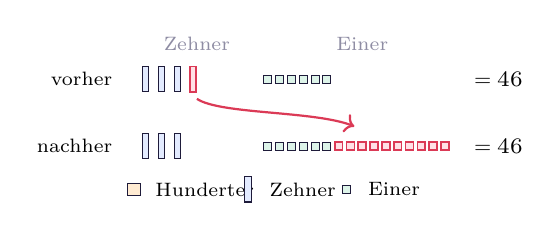
\begin{tikzpicture}[baseline=(current bounding box.north),font=\scriptsize]
  \node[text=pxgray] at (2.0,0.85) {Zehner}; \node[text=pxgray] at (4.1,0.85) {Einer};
  \node[anchor=east] at (1.05,0.4) {vorher}; \node[anchor=east] at (1.05,-0.45) {nachher};
  \foreach \pxbi in {1,2,3}{\pxsymZ{1.15+\pxbi*0.2}{0.4}}
  \pxsymZ[px hi]{1.15+4*0.2}{0.4}
  \foreach \pxbi in {1,...,6}{\pxsymE{2.75+\pxbi*0.15}{0.4}}
  \node[anchor=west,font=\footnotesize\bfseries] at (5.4,0.4) {$=46$};
  \foreach \pxbi in {1,2,3}{\pxsymZ{1.15+\pxbi*0.2}{-0.45}}
  \foreach \pxbi in {1,...,6}{\pxsymE{2.75+\pxbi*0.15}{-0.45}}
  \foreach \pxbi in {7,...,16}{\pxsymE[px hi]{2.75+\pxbi*0.15}{-0.45}}
  \node[anchor=west,font=\footnotesize\bfseries] at (5.4,-0.45) {$=46$};
  \draw[->,line width=0.8pt,pxred] (2.0,0.15) .. controls (2.3,-0.05) and (3.5,0.0) .. (4.0,-0.2);
  \pxlegende{1.2}{-1.0}
\end{tikzpicture}}

% \buendelnull = Entbündeln über eine Null als Stellenwerttafel in drei Zeilen am Beispiel 800:
%   vorher 8 H -> 1 H = 10 Z: 7 H + 10 Z -> 2 Z = 20 E: 7 H + 8 Z + 20 E (immer 800). Getauschtes rot. Komplett-Kürzel, ca. 7 cm breit.
\newcommand{\buendelnull}{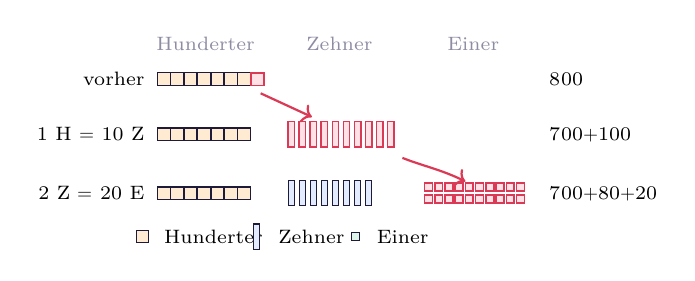
\begin{tikzpicture}[baseline=(current bounding box.north),font=\scriptsize]
  \node[text=pxgray] at (2.0,0.95) {Hunderter}; \node[text=pxgray] at (3.7,0.95) {Zehner}; \node[text=pxgray] at (5.4,0.95) {Einer};
  \node[anchor=east] at (1.35,0.5) {vorher}; \node[anchor=east] at (1.35,-0.2) {1 H $=$ 10 Z}; \node[anchor=east] at (1.35,-0.95) {2 Z $=$ 20 E};
  % Zeile 1: 800
  \foreach \pxbi in {1,...,7}{\pxsymH{1.3+\pxbi*0.17}{0.5}}
  \pxsymH[px hi]{1.3+8*0.17}{0.5}
  \node[anchor=west,font=\scriptsize\bfseries] at (6.25,0.5) {$800$};
  % Zeile 2: 7 H + 10 Z
  \foreach \pxbi in {1,...,7}{\pxsymH{1.3+\pxbi*0.17}{-0.2}}
  \foreach \pxbi in {1,...,10}{\pxsymZ[px hi]{2.95+\pxbi*0.14}{-0.2}}
  \node[anchor=west,font=\scriptsize\bfseries] at (6.25,-0.2) {$700{+}100$};
  % Zeile 3: 7 H + 8 Z + 20 E
  \foreach \pxbi in {1,...,7}{\pxsymH{1.3+\pxbi*0.17}{-0.95}}
  \foreach \pxbi in {1,...,8}{\pxsymZ{2.95+\pxbi*0.14}{-0.95}}
  \foreach \pxbi in {1,...,10}{\pxsymE[px hi]{4.7+\pxbi*0.13}{-0.87}\pxsymE[px hi]{4.7+\pxbi*0.13}{-1.02}}
  \node[anchor=west,font=\scriptsize\bfseries] at (6.25,-0.95) {$700{+}80{+}20$};
  \draw[->,line width=0.8pt,pxred] (2.7,0.32) -- (3.35,0.02);
  \draw[->,line width=0.8pt,pxred] (4.5,-0.5) .. controls (4.75,-0.6) and (5.0,-0.65) .. (5.3,-0.8);
  \pxlegende{1.2}{-1.5}
\end{tikzpicture}}

% \uebertragbild = Idee hinter dem Übertrag beim Ergänzen am Beispiel 46-37: Im Einer geht 6-7 nicht.
%   Oben kommen 10 Einer dazu (rot), unten 1 Zehner = 10 Einer (rot): beide Zahlen werden gleich viel größer, der Abstand (9) bleibt.
%   Stellenwerttafel vorher/nachher, oben = 46, unten = 37. Komplett-Kürzel, ca. 7 cm breit.
\newcommand{\uebertragbild}{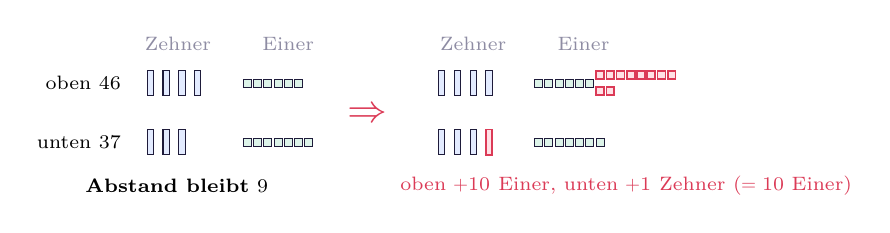
\begin{tikzpicture}[baseline=(current bounding box.north),font=\scriptsize]
  \node[text=pxgray] at (1.35,0.95) {Zehner}; \node[text=pxgray] at (2.75,0.95) {Einer};
  \node[text=pxgray] at (5.1,0.95) {Zehner}; \node[text=pxgray] at (6.5,0.95) {Einer};
  \node[anchor=east] at (0.75,0.45) {oben 46}; \node[anchor=east] at (0.75,-0.3) {unten 37};
  % vorher
  \foreach \pxbi in {1,...,4}{\pxsymZ{0.8+\pxbi*0.2}{0.45}}
  \foreach \pxbi in {1,...,6}{\pxsymE{2.1+\pxbi*0.13}{0.45}}
  \foreach \pxbi in {1,...,3}{\pxsymZ{0.8+\pxbi*0.2}{-0.3}}
  \foreach \pxbi in {1,...,7}{\pxsymE{2.1+\pxbi*0.13}{-0.3}}
  \node[font=\Large,text=pxred] at (3.75,0.08) {$\Rightarrow$};
  % nachher
  \foreach \pxbi in {1,...,4}{\pxsymZ{4.5+\pxbi*0.2}{0.45}}
  \foreach \pxbi in {1,...,6}{\pxsymE{5.8+\pxbi*0.13}{0.45}}
  \foreach \pxbi in {7,...,14}{\pxsymE[px hi]{5.8+\pxbi*0.13}{0.55}}
  \foreach \pxbi in {15,...,16}{\pxsymE[px hi]{5.8+\pxbi*0.13-8*0.13}{0.35}}
  \foreach \pxbi in {1,...,3}{\pxsymZ{4.5+\pxbi*0.2}{-0.3}}
  \pxsymZ[px hi]{4.5+4*0.2}{-0.3}
  \foreach \pxbi in {1,...,7}{\pxsymE{5.8+\pxbi*0.13}{-0.3}}
  \node[text=pxred,anchor=west] at (4.05,-0.85) {oben $+10$ Einer, unten $+1$ Zehner ($=10$ Einer)};
  \node[anchor=west,font=\scriptsize\bfseries] at (0.05,-0.85) {Abstand bleibt $9$};
\end{tikzpicture}}

% \ergaenzenstrahl = Ergänzen: Summe 13 bis 20 ergänzen (Sprung +7), 20 sind zwei Zehner = Übertrag 2. Komplett-Kürzel, ca. 7 cm breit.
\newcommand{\ergaenzenstrahl}{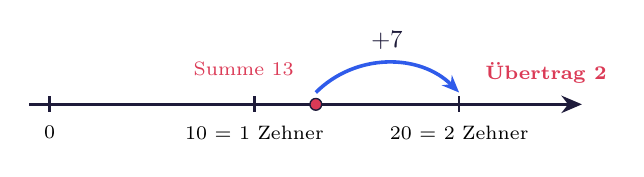
\begin{tikzpicture}[x=0.26cm,y=1cm,baseline=(current bounding box.north),font=\scriptsize]
  \draw[px axis] (-1,0) -- (26,0);
  \foreach \pxai/\pxat in {0/0,10/{10 = 1 Zehner},20/{20 = 2 Zehner}}{\draw[px tick] (\pxai,0.1) -- (\pxai,-0.1); \node[below=0.5mm,align=center,font=\scriptsize] at (\pxai,-0.1) {\pxat};}
  \node[px pt,inner sep=1.5pt,circle,draw=pxink,fill=pxred] at (13,0) {}; \node[anchor=east,text=pxred] at (12.4,0.45) {Summe 13};
  \draw[px jump] (13,0.15) to[bend left=45] node[px jlab,midway,above=1mm]{$+7$} (20,0.15);
  \node[text=pxred,anchor=west,font=\scriptsize\bfseries] at (20.8,0.4) {Übertrag 2};
\end{tikzpicture}}

% ---------- Rechenschritte in Sprechblasen ----------
% \schrittbildentb / \schrittbilderg: Rechnung 846-213-124 untereinander, Einerstelle mit nummerierten Sprechblasen
% (Entbündeln bzw. Ergänzen). Komplett-Kürzel, ca. 7,5 cm breit. Text der Blasen ist im Kürzel festgelegt.
\tikzset{px bubble/.style={rectangle callout,rounded corners=2pt,draw=pxpurple,fill=white,line width=0.6pt,text width=3.55cm,font=\scriptsize,inner sep=2.2pt,align=left,callout pointer width=0.15cm},
  px bubblepic/.style={rectangle callout,rounded corners=2pt,draw=pxpurple,fill=white,line width=0.6pt,inner sep=2pt,callout pointer width=0.15cm},
  px mark/.style={draw=pxpurple,rounded corners=2pt,line width=0.7pt,dashed}}
\newcommand{\pxnum}[1]{\tikz[baseline=-0.6ex]{\node[circle,fill=pxpurple,text=white,inner sep=1pt,font=\tiny\bfseries] {#1};}}
% \buendelbildklein / \uebertragbildklein: kleine Fassungen (ca. 3,8 cm breit) für Sprechblasen; Beispiel 46 bzw. 46-37
\newcommand{\buendelbildklein}{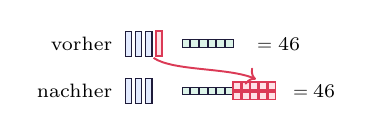
\begin{tikzpicture}[font=\scriptsize]
  \node[anchor=east] at (0.65,0.3) {vorher}; \node[anchor=east] at (0.65,-0.3) {nachher};
  \foreach \pxbi in {1,2,3}{\pxsymZ{0.6+\pxbi*0.13}{0.3}} \pxsymZ[px hi]{0.6+4*0.13}{0.3}
  \foreach \pxbi in {1,...,6}{\pxsymE{1.35+\pxbi*0.11}{0.3}}
  \node[anchor=west] at (2.25,0.3) {$=46$};
  \foreach \pxbi in {1,2,3}{\pxsymZ{0.6+\pxbi*0.13}{-0.3}}
  \foreach \pxbi in {1,...,6}{\pxsymE{1.35+\pxbi*0.11}{-0.3}}
  \foreach \pxbi in {1,...,5}{\pxsymE[px hi]{2.0+\pxbi*0.11}{-0.24}\pxsymE[px hi]{2.0+\pxbi*0.11}{-0.36}}
  \node[anchor=west] at (2.7,-0.3) {$=46$};
  \draw[->,line width=0.7pt,pxred] (1.05,0.12) .. controls (1.3,-0.05) and (2.0,0.0) .. (2.35,-0.15);
\end{tikzpicture}}
\newcommand{\uebertragbildklein}{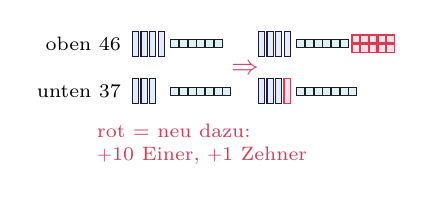
\begin{tikzpicture}[baseline=(current bounding box.south),font=\scriptsize]
  \node[anchor=east] at (0.6,0.3) {oben 46}; \node[anchor=east] at (0.6,-0.3) {unten 37};
  \foreach \pxbi in {1,...,4}{\pxsymZ{0.55+\pxbi*0.11}{0.3}} \foreach \pxbi in {1,...,6}{\pxsymE{1.05+\pxbi*0.11}{0.3}}
  \foreach \pxbi in {1,...,3}{\pxsymZ{0.55+\pxbi*0.11}{-0.3}} \foreach \pxbi in {1,...,7}{\pxsymE{1.05+\pxbi*0.11}{-0.3}}
  \node[font=\normalsize,text=pxred] at (2.05,0) {$\Rightarrow$};
  \foreach \pxbi in {1,...,4}{\pxsymZ{2.15+\pxbi*0.11}{0.3}} \foreach \pxbi in {1,...,6}{\pxsymE{2.65+\pxbi*0.11}{0.3}}
  \foreach \pxbi in {1,...,5}{\pxsymE[px hi]{3.35+\pxbi*0.11}{0.36}\pxsymE[px hi]{3.35+\pxbi*0.11}{0.24}}
  \foreach \pxbi in {1,...,3}{\pxsymZ{2.15+\pxbi*0.11}{-0.3}} \pxsymZ[px hi]{2.15+4*0.11}{-0.3}
  \foreach \pxbi in {1,...,7}{\pxsymE{2.65+\pxbi*0.11}{-0.3}}
  \node[text=pxred,anchor=north west,align=left] at (0.05,-0.6) {rot = neu dazu:\\$+10$ Einer, $+1$ Zehner};
\end{tikzpicture}}

\newcommand{\schrittbildentb}{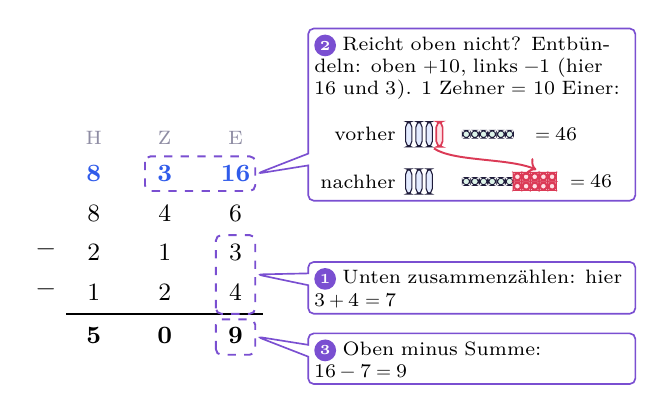
\begin{tikzpicture}[baseline=(current bounding box.north),font=\small]
  \foreach \pxsx/\pxst in {0.9/H,1.8/Z,2.7/E}{\node[text=pxgray,font=\scriptsize] at (\pxsx,0.45) {\pxst};}
  \node[text=pxblue,font=\small\bfseries] at (0.9,0) {8}; \node[text=pxblue,font=\small\bfseries] at (1.8,0) {3}; \node[text=pxblue,font=\small\bfseries] at (2.7,0) {16};
  \node at (0.9,-0.5) {8}; \node at (1.8,-0.5) {4}; \node at (2.7,-0.5) {6};
  \node at (0.3,-1.0) {$-$}; \node at (0.9,-1.0) {2}; \node at (1.8,-1.0) {1}; \node at (2.7,-1.0) {3};
  \node at (0.3,-1.5) {$-$}; \node at (0.9,-1.5) {1}; \node at (1.8,-1.5) {2}; \node at (2.7,-1.5) {4};
  \draw[line width=0.6pt] (0.55,-1.78) -- (3.05,-1.78);
  \node[font=\small\bfseries] at (0.9,-2.05) {5}; \node[font=\small\bfseries] at (1.8,-2.05) {0}; \node[font=\small\bfseries] at (2.7,-2.05) {9};
  \draw[px mark] (2.45,-1.78) rectangle (2.95,-0.78);
  \draw[px mark] (1.55,0.22) rectangle (2.95,-0.22);
  \draw[px mark] (2.45,-2.3) rectangle (2.95,-1.85);
  \node[px bubble,text width=4.0cm,callout absolute pointer={(2.97,0)}] at (5.7,0.75) {\pxnum{2} Reicht oben nicht? Entbündeln: oben \mbox{$+10$}, links \mbox{$-1$} (hier $16$ und $3$). $1$ Zehner $=$ $10$ Einer:\par\vspace{0.5mm}\buendelbildklein};
  \node[px bubble,text width=4.0cm,callout absolute pointer={(2.97,-1.28)}] at (5.7,-1.45) {\pxnum{1} Unten zusammenzählen: hier \mbox{$3+4=7$}};
  \node[px bubble,text width=4.0cm,callout absolute pointer={(2.97,-2.07)}] at (5.7,-2.35) {\pxnum{3} Oben minus Summe: \mbox{$16-7=9$}};
\end{tikzpicture}}
\newcommand{\schrittbilderg}{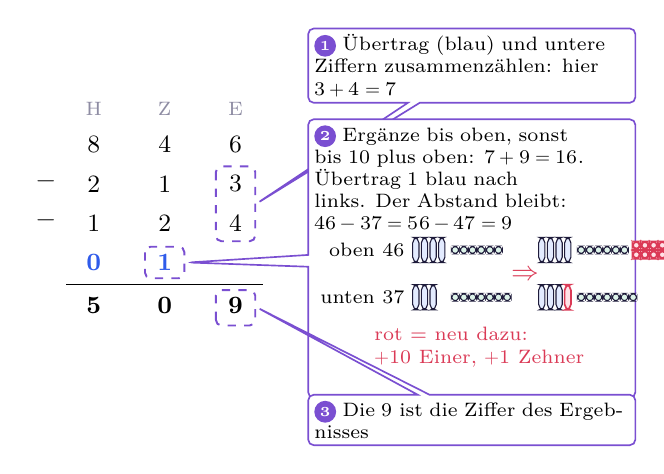
\begin{tikzpicture}[baseline=(current bounding box.north),font=\small]
  \foreach \pxsx/\pxst in {0.9/H,1.8/Z,2.7/E}{\node[text=pxgray,font=\scriptsize] at (\pxsx,0.45) {\pxst};}
  \node at (0.9,0) {8}; \node at (1.8,0) {4}; \node at (2.7,0) {6};
  \node at (0.3,-0.5) {$-$}; \node at (0.9,-0.5) {2}; \node at (1.8,-0.5) {1}; \node at (2.7,-0.5) {3};
  \node at (0.3,-1.0) {$-$}; \node at (0.9,-1.0) {1}; \node at (1.8,-1.0) {2}; \node at (2.7,-1.0) {4};
  \node[text=pxblue,font=\small\bfseries] at (0.9,-1.5) {0}; \node[text=pxblue,font=\small\bfseries] at (1.8,-1.5) {1};
  \draw[line width=0.6pt] (0.55,-1.78) -- (3.05,-1.78);
  \node[font=\small\bfseries] at (0.9,-2.05) {5}; \node[font=\small\bfseries] at (1.8,-2.05) {0}; \node[font=\small\bfseries] at (2.7,-2.05) {9};
  \draw[px mark] (2.45,-0.28) rectangle (2.95,-1.23);
  \draw[px mark] (1.55,-1.3) rectangle (2.05,-1.7);
  \draw[px mark] (2.45,-2.3) rectangle (2.95,-1.85);
  \node[px bubble,text width=4.0cm,callout absolute pointer={(2.97,-0.75)}] at (5.7,1.0) {\pxnum{1} Übertrag (blau) und untere Ziffern zusammenzählen: hier \mbox{$3+4=7$}};
  \node[px bubble,text width=4.0cm,callout absolute pointer={(2.1,-1.5)}] at (5.7,-1.45) {\pxnum{2} Ergänze bis oben, sonst bis $10$ plus oben: \mbox{$7+9=16$}. Übertrag $1$ blau nach links. Der Abstand bleibt: \mbox{$46-37=56-47=9$}\par\vspace{0.5mm}\uebertragbildklein};
  \node[px bubble,text width=4.0cm,callout absolute pointer={(2.97,-2.07)}] at (5.7,-3.5) {\pxnum{3} Die $9$ ist die Ziffer des Ergebnisses};
\end{tikzpicture}}

% \schrittbildnullentb / \schrittbildnullerg: 800-256-317 untereinander, daneben die Skizze in einer Sprechblase,
% die auf die Stelle zeigt, an der getauscht bzw. der Übertrag gebildet wird. Komplett-Kürzel, ca. 7,5 cm breit.
\newcommand{\schrittbildnullentb}{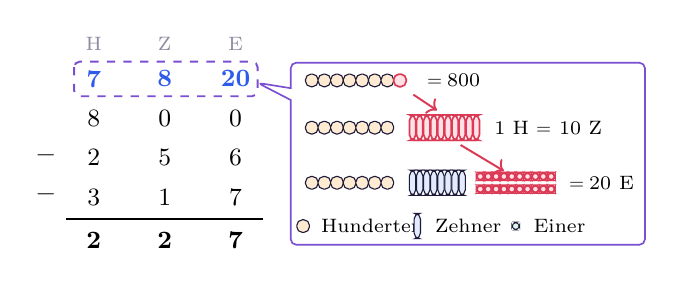
\begin{tikzpicture}[baseline=(current bounding box.north),font=\small]
  \foreach \pxsx/\pxst in {0.9/H,1.8/Z,2.7/E}{\node[text=pxgray,font=\scriptsize] at (\pxsx,0.45) {\pxst};}
  \node[text=pxblue,font=\small\bfseries] at (0.9,0) {7}; \node[text=pxblue,font=\small\bfseries] at (1.8,0) {8}; \node[text=pxblue,font=\small\bfseries] at (2.7,0) {20};
  \node at (0.9,-0.5) {8}; \node at (1.8,-0.5) {0}; \node at (2.7,-0.5) {0};
  \node at (0.3,-1.0) {$-$}; \node at (0.9,-1.0) {2}; \node at (1.8,-1.0) {5}; \node at (2.7,-1.0) {6};
  \node at (0.3,-1.5) {$-$}; \node at (0.9,-1.5) {3}; \node at (1.8,-1.5) {1}; \node at (2.7,-1.5) {7};
  \draw[line width=0.6pt] (0.55,-1.78) -- (3.05,-1.78);
  \node[font=\small\bfseries] at (0.9,-2.05) {2}; \node[font=\small\bfseries] at (1.8,-2.05) {2}; \node[font=\small\bfseries] at (2.7,-2.05) {7};
  \draw[px mark] (0.65,0.22) rectangle (2.98,-0.22);
  \node[px bubblepic,callout absolute pointer={(2.98,-0.05)}] at (5.65,-0.95) {\buendelnullklein};
\end{tikzpicture}}
\newcommand{\schrittbildnullerg}{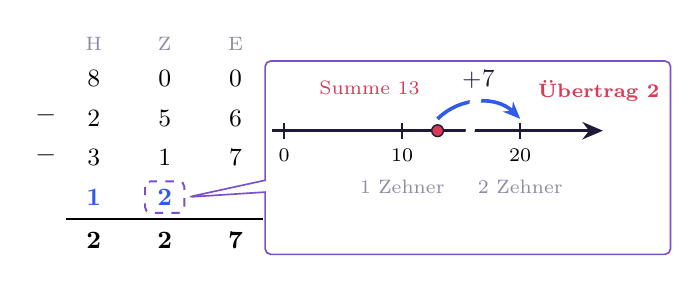
\begin{tikzpicture}[baseline=(current bounding box.north),font=\small]
  \foreach \pxsx/\pxst in {0.9/H,1.8/Z,2.7/E}{\node[text=pxgray,font=\scriptsize] at (\pxsx,0.45) {\pxst};}
  \node at (0.9,0) {8}; \node at (1.8,0) {0}; \node at (2.7,0) {0};
  \node at (0.3,-0.5) {$-$}; \node at (0.9,-0.5) {2}; \node at (1.8,-0.5) {5}; \node at (2.7,-0.5) {6};
  \node at (0.3,-1.0) {$-$}; \node at (0.9,-1.0) {3}; \node at (1.8,-1.0) {1}; \node at (2.7,-1.0) {7};
  \node[text=pxblue,font=\small\bfseries] at (0.9,-1.5) {1}; \node[text=pxblue,font=\small\bfseries] at (1.8,-1.5) {2};
  \draw[line width=0.6pt] (0.55,-1.78) -- (3.05,-1.78);
  \node[font=\small\bfseries] at (0.9,-2.05) {2}; \node[font=\small\bfseries] at (1.8,-2.05) {2}; \node[font=\small\bfseries] at (2.7,-2.05) {7};
  \draw[px mark] (1.55,-1.3) rectangle (2.05,-1.7);
  \node[px bubblepic,callout absolute pointer={(2.1,-1.5)}] at (5.65,-1.0) {\ergaenzenstrahlklein};
\end{tikzpicture}}

% \buendelnullklein / \ergaenzenstrahlklein: kleine Fassungen (ca. 4,3 cm breit, gleiche Schriftgröße wie sonst) für die Sprechblasen neben der Rechnung
\newcommand{\buendelnullklein}{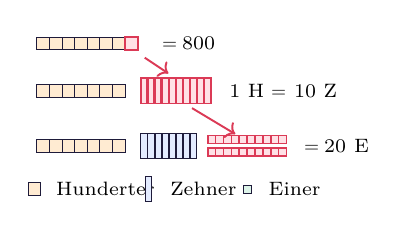
\begin{tikzpicture}[font=\scriptsize]
  \foreach \pxbi in {1,...,7}{\pxsymH{\pxbi*0.16}{0.6}} \pxsymH[px hi]{8*0.16}{0.6}
  \node[anchor=west] at (1.55,0.6) {$=800$};
  \foreach \pxbi in {1,...,7}{\pxsymH{\pxbi*0.16}{0}}
  \foreach \pxbi in {1,...,10}{\pxsymZ[px hi]{1.35+\pxbi*0.09}{0}}
  \node[anchor=west] at (2.4,0) {1 H $=$ 10 Z};
  \foreach \pxbi in {1,...,7}{\pxsymH{\pxbi*0.16}{-0.7}}
  \foreach \pxbi in {1,...,8}{\pxsymZ{1.35+\pxbi*0.09}{-0.7}}
  \foreach \pxbi in {1,...,10}{\pxsymE[px hi]{2.2+\pxbi*0.1}{-0.62}\pxsymE[px hi]{2.2+\pxbi*0.1}{-0.78}}
  \node[anchor=west] at (3.35,-0.7) {$=20$ E};
  \draw[->,line width=0.7pt,pxred] (1.45,0.42) -- (1.75,0.22);
  \draw[->,line width=0.7pt,pxred] (2.05,-0.22) -- (2.6,-0.55);
  \pxlegende{0.05}{-1.25}
\end{tikzpicture}}
\newcommand{\ergaenzenstrahlklein}{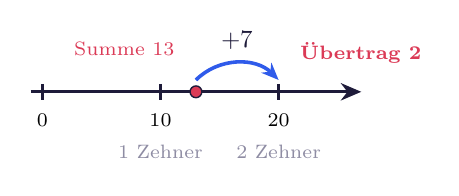
\begin{tikzpicture}[x=0.15cm,y=1cm,font=\scriptsize]
  \draw[px axis] (-1,0) -- (27,0);
  \foreach \pxai/\pxat in {0/0,10/{10},20/{20}}{\draw[px tick] (\pxai,0.1) -- (\pxai,-0.1); \node[below=0.5mm] at (\pxai,-0.1) {\pxat};}
  \node[below=0.5mm,text=pxgray] at (10,-0.5) {1 Zehner}; \node[below=0.5mm,text=pxgray] at (20,-0.5) {2 Zehner};
  \node[px pt,inner sep=1.5pt,circle,draw=pxink,fill=pxred] at (13,0) {}; \node[anchor=east,text=pxred] at (12,0.55) {Summe 13};
  \draw[px jump] (13,0.15) to[bend left=45] node[px jlab,midway,above=1mm]{$+7$} (20,0.15);
  \node[text=pxred,anchor=west,font=\scriptsize\bfseries] at (21,0.5) {Übertrag 2};
\end{tikzpicture}}

% Zwei Spalten mit senkrechtem Trennstrich (z. B. Entbündeln links, Ergänzen rechts): \zweispalten{links}{rechts}
\newcommand{\zweispalten}[2]{\par\noindent{\setlength{\tabcolsep}{0pt}\begin{tabular}{@{}p{0.465\linewidth}@{\hspace{3mm}}!{\color{pxgray}\vrule width 0.7pt}@{\hspace{3mm}}p{0.465\linewidth}@{}}#1&#2\end{tabular}}\par}

% Zentrierte Zeichnungen mit knapperem Abstand
\renewenvironment{center}{\par\begingroup\setlength{\topsep}{1mm plus 1mm}\setlength{\partopsep}{0pt}\trivlist\centering\item\relax}{\endtrivlist\endgroup}
\AtBeginDocument{\setlength{\parskip}{0.36em}}

% Name/Datum: Deckblatt (über dem Titel) und Kopf der geraden Seiten (Rückseite)
\makeatletter
\fancyhead[L]{\ifexamshownameheader\ifnum\value{page}>1\ifodd\value{page}\else\footnotesize\textbf{Name:}\ \rule{4.6cm}{0.4pt}\quad\textbf{Datum:}\ \rule{2.4cm}{0.4pt}\fi\fi\fi}
\fancyhead[R]{\ifnum\value{page}>1\ifodd\value{page}\else\footnotesize\color{gray}Seite \thepage\fi\fi}
\makeatother

% ==========================================================================
% ERKLÄRBILDER für "Schritt für Schritt"-Kästen (\algobox): Rechnung mit nummerierten Sprechblasen und Skizzen.
% Komplett-Kürzel, jeweils ca. 7,7 cm breit (passen in \zweispalten). Skizzen in Blasen wie in \schrittbildentb.
% ==========================================================================
% --- Subtraktion, ein Subtrahend: 846-237 (Einerstelle, Skizzen 46 und 46-37) ---
\newcommand{\schrittbildentbeins}{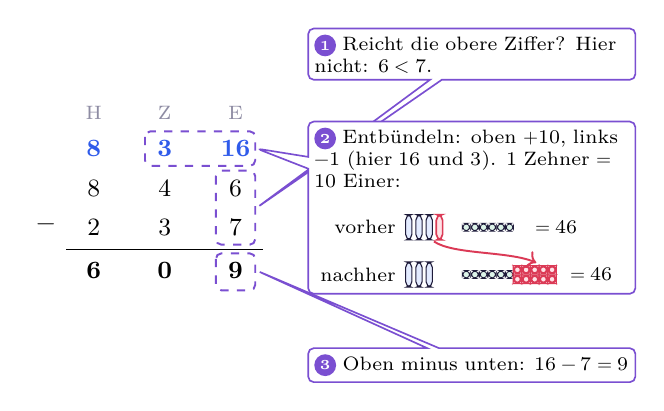
\begin{tikzpicture}[baseline=(current bounding box.north),font=\small]
  \foreach \pxsx/\pxst in {0.9/H,1.8/Z,2.7/E}{\node[text=pxgray,font=\scriptsize] at (\pxsx,0.45) {\pxst};}
  \node[text=pxblue,font=\small\bfseries] at (0.9,0) {8}; \node[text=pxblue,font=\small\bfseries] at (1.8,0) {3}; \node[text=pxblue,font=\small\bfseries] at (2.7,0) {16};
  \node at (0.9,-0.5) {8}; \node at (1.8,-0.5) {4}; \node at (2.7,-0.5) {6};
  \node at (0.3,-1.0) {$-$}; \node at (0.9,-1.0) {2}; \node at (1.8,-1.0) {3}; \node at (2.7,-1.0) {7};
  \draw[line width=0.6pt] (0.55,-1.28) -- (3.05,-1.28);
  \node[font=\small\bfseries] at (0.9,-1.55) {6}; \node[font=\small\bfseries] at (1.8,-1.55) {0}; \node[font=\small\bfseries] at (2.7,-1.55) {9};
  \draw[px mark] (2.45,-0.28) rectangle (2.95,-1.22);
  \draw[px mark] (1.55,0.22) rectangle (2.95,-0.22);
  \draw[px mark] (2.45,-1.33) rectangle (2.95,-1.8);
  \node[px bubble,text width=4.0cm,callout absolute pointer={(2.97,-0.75)}] at (5.7,1.2) {\pxnum{1} Reicht die obere Ziffer? Hier nicht: $6<7$.};
  \node[px bubble,text width=4.0cm,callout absolute pointer={(2.97,0)}] at (5.7,-0.75) {\pxnum{2} Entbündeln: oben \mbox{$+10$}, links \mbox{$-1$} (hier $16$ und $3$). $1$ Zehner $=$ $10$ Einer:\par\vspace{0.5mm}\buendelbildklein};
  \node[px bubble,text width=4.0cm,callout absolute pointer={(2.97,-1.55)}] at (5.7,-2.75) {\pxnum{3} Oben minus unten: \mbox{$16-7=9$}};
\end{tikzpicture}}
\newcommand{\schrittbildergeins}{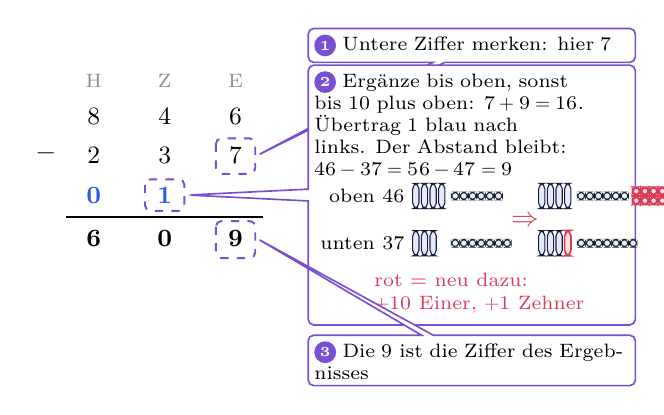
\begin{tikzpicture}[baseline=(current bounding box.north),font=\small]
  \foreach \pxsx/\pxst in {0.9/H,1.8/Z,2.7/E}{\node[text=pxgray,font=\scriptsize] at (\pxsx,0.45) {\pxst};}
  \node at (0.9,0) {8}; \node at (1.8,0) {4}; \node at (2.7,0) {6};
  \node at (0.3,-0.5) {$-$}; \node at (0.9,-0.5) {2}; \node at (1.8,-0.5) {3}; \node at (2.7,-0.5) {7};
  \node[text=pxblue,font=\small\bfseries] at (0.9,-1.0) {0}; \node[text=pxblue,font=\small\bfseries] at (1.8,-1.0) {1};
  \draw[line width=0.6pt] (0.55,-1.28) -- (3.05,-1.28);
  \node[font=\small\bfseries] at (0.9,-1.55) {6}; \node[font=\small\bfseries] at (1.8,-1.55) {0}; \node[font=\small\bfseries] at (2.7,-1.55) {9};
  \draw[px mark] (2.45,-0.28) rectangle (2.95,-0.73);
  \draw[px mark] (1.55,-0.8) rectangle (2.05,-1.2);
  \draw[px mark] (2.45,-1.33) rectangle (2.95,-1.8);
  \node[px bubble,text width=4.0cm,callout absolute pointer={(2.97,-0.5)}] at (5.7,0.9) {\pxnum{1} Untere Ziffer merken: hier $7$};
  \node[px bubble,text width=4.0cm,callout absolute pointer={(2.1,-1.0)}] at (5.7,-1.0) {\pxnum{2} Ergänze bis oben, sonst bis $10$ plus oben: \mbox{$7+9=16$}. Übertrag $1$ blau nach links. Der Abstand bleibt: \mbox{$46-37=56-47=9$}\par\vspace{0.5mm}\uebertragbildklein};
  \node[px bubble,text width=4.0cm,callout absolute pointer={(2.97,-1.55)}] at (5.7,-3.1) {\pxnum{3} Die $9$ ist die Ziffer des Ergebnisses};
\end{tikzpicture}}
% --- Multiplikation: 143*6 (Bündeln 18 = 1 Z 8 E) und 326*24 (zwei Teilprodukte) ---
\newcommand{\buendelmalklein}{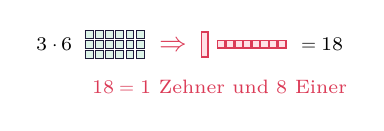
\begin{tikzpicture}[baseline=(current bounding box.south),font=\scriptsize]
  \foreach \pxr in {1,2,3}{\foreach \pxc in {1,...,6}{\pxsymE{\pxc*0.13}{-\pxr*0.13+0.5}}}
  \node[anchor=east] at (0.05,0.24) {$3\cdot6$};
  \node[font=\normalsize,text=pxred] at (1.2,0.24) {$\Rightarrow$};
  \pxsymZ[px hi]{1.6}{0.24}
  \foreach \pxc in {1,...,8}{\pxsymE[px hi]{1.7+\pxc*0.11}{0.24}}
  \node[anchor=west] at (2.7,0.24) {$=18$};
  \node[text=pxred,anchor=west] at (0.05,-0.3) {$18=1$ Zehner und $8$ Einer};
\end{tikzpicture}}
\newcommand{\schrittbildmal}{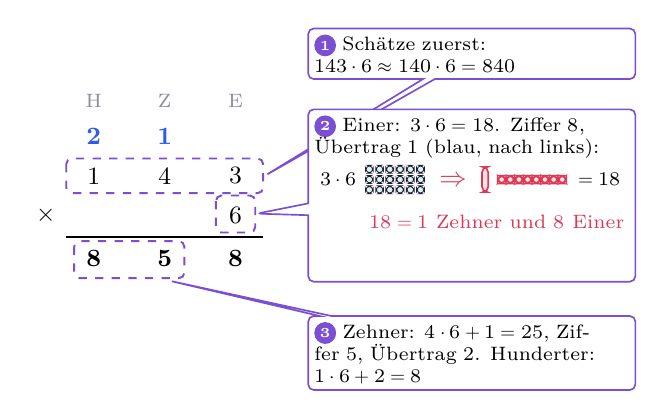
\begin{tikzpicture}[baseline=(current bounding box.north),font=\small]
  \foreach \pxsx/\pxst in {0.9/H,1.8/Z,2.7/E}{\node[text=pxgray,font=\scriptsize] at (\pxsx,0.45) {\pxst};}
  \node[text=pxblue,font=\small\bfseries] at (0.9,0) {2}; \node[text=pxblue,font=\small\bfseries] at (1.8,0) {1};
  \node at (0.9,-0.5) {1}; \node at (1.8,-0.5) {4}; \node at (2.7,-0.5) {3};
  \node at (0.3,-1.0) {$\times$}; \node at (2.7,-1.0) {6};
  \draw[line width=0.6pt] (0.55,-1.28) -- (3.05,-1.28);
  \node[font=\small\bfseries] at (0.9,-1.55) {8}; \node[font=\small\bfseries] at (1.8,-1.55) {5}; \node[font=\small\bfseries] at (2.7,-1.55) {8};
  \draw[px mark] (0.55,-0.28) rectangle (3.05,-0.72);
  \draw[px mark] (2.45,-0.75) rectangle (2.95,-1.22);
  \draw[px mark] (0.65,-1.33) rectangle (2.05,-1.8);
  \node[px bubble,text width=4.0cm,callout absolute pointer={(3.07,-0.5)}] at (5.7,1.05) {\pxnum{1} Schätze zuerst: \mbox{$143\cdot6\approx140\cdot6=840$}};
  \node[px bubble,text width=4.0cm,callout absolute pointer={(2.97,-0.98)}] at (5.7,-0.75) {\pxnum{2} Einer: \mbox{$3\cdot6=18$}. Ziffer $8$, Übertrag $1$ (blau, nach links):\par\vspace{0.5mm}\buendelmalklein};
  \node[px bubble,text width=4.0cm,callout absolute pointer={(1.85,-1.83)}] at (5.7,-2.75) {\pxnum{3} Zehner: \mbox{$4\cdot6+1=25$}, Ziffer $5$, Übertrag $2$. Hunderter: \mbox{$1\cdot6+2=8$}};
\end{tikzpicture}}
% Warum der Übertrag: 143*6 als Malkreuz-Streifen (600 + 240 + 18)
\newcommand{\malstreifen}{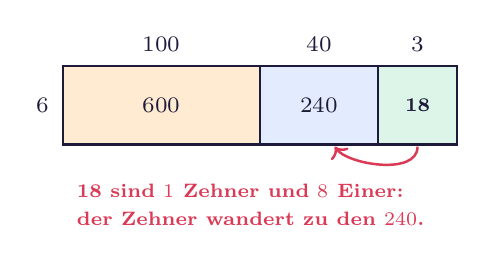
\begin{tikzpicture}[x=0.5cm,y=0.5cm,baseline=(current bounding box.north),font=\small]
  \fteil{0}{0}{5}{2}{px bar b}{$600$}\fteil{5}{0}{8}{2}{px bar}{$240$}\fteil{8}{0}{10}{2}{px bar c}{\scriptsize 18}
  \foben{2.5}{2}{$100$}\foben{6.5}{2}{$40$}\foben{9}{2}{$3$}\flinks{0}{1}{$6$}
  \draw[->,line width=0.9pt,pxred] (9,-0.05) .. controls (9,-0.8) and (7.2,-0.5) .. (6.9,-0.05);
  \node[px note,text=pxred,anchor=north west,font=\scriptsize\bfseries] at (0.1,-0.75) {18 sind $1$ Zehner und $8$ Einer:};
  \node[px note,text=pxred,anchor=north west,font=\scriptsize\bfseries] at (0.1,-1.45) {der Zehner wandert zu den $240$.};
\end{tikzpicture}}
\newcommand{\schrittbildmalzwei}{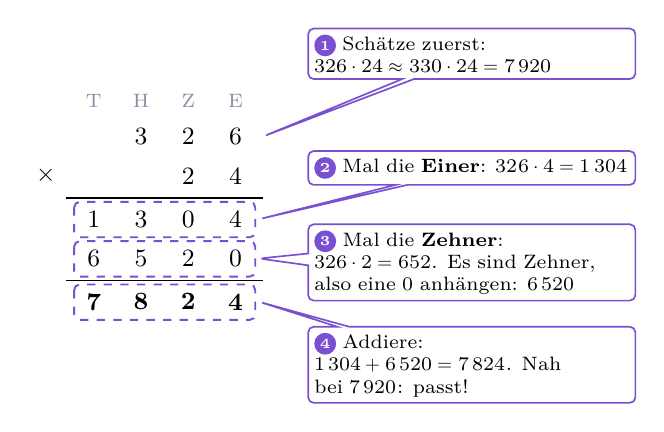
\begin{tikzpicture}[baseline=(current bounding box.north),font=\small]
  \foreach \pxsx/\pxst in {0.9/T,1.5/H,2.1/Z,2.7/E}{\node[text=pxgray,font=\scriptsize] at (\pxsx,0.45) {\pxst};}
  \node at (1.5,0) {3}; \node at (2.1,0) {2}; \node at (2.7,0) {6};
  \node at (0.3,-0.5) {$\times$}; \node at (2.1,-0.5) {2}; \node at (2.7,-0.5) {4};
  \draw[line width=0.6pt] (0.55,-0.78) -- (3.05,-0.78);
  \node at (0.9,-1.05) {1}; \node at (1.5,-1.05) {3}; \node at (2.1,-1.05) {0}; \node at (2.7,-1.05) {4};
  \node at (0.9,-1.55) {6}; \node at (1.5,-1.55) {5}; \node at (2.1,-1.55) {2}; \node at (2.7,-1.55) {0};
  \draw[line width=0.6pt] (0.55,-1.83) -- (3.05,-1.83);
  \node[font=\small\bfseries] at (0.9,-2.1) {7}; \node[font=\small\bfseries] at (1.5,-2.1) {8}; \node[font=\small\bfseries] at (2.1,-2.1) {2}; \node[font=\small\bfseries] at (2.7,-2.1) {4};
  \draw[px mark] (0.65,-0.83) rectangle (2.95,-1.28);
  \draw[px mark] (0.65,-1.33) rectangle (2.95,-1.78);
  \draw[px mark] (0.65,-1.88) rectangle (2.95,-2.33);
  \node[px bubble,text width=4.0cm,callout absolute pointer={(3.05,0)}] at (5.7,1.05) {\pxnum{1} Schätze zuerst: \mbox{$326\cdot24\approx330\cdot24=7\,920$}};
  \node[px bubble,text width=4.0cm,callout absolute pointer={(3.0,-1.05)}] at (5.7,-0.4) {\pxnum{2} Mal die \textbf{Einer}: \mbox{$326\cdot4=1\,304$}};
  \node[px bubble,text width=4.0cm,callout absolute pointer={(3.0,-1.55)}] at (5.7,-1.6) {\pxnum{3} Mal die \textbf{Zehner}: \mbox{$326\cdot2=652$}. Es sind Zehner, also eine $0$ anhängen: $6\,520$};
  \node[px bubble,text width=4.0cm,callout absolute pointer={(3.0,-2.1)}] at (5.7,-2.9) {\pxnum{4} Addiere: \mbox{$1\,304+6\,520=7\,824$}. Nah bei $7\,920$: passt!};
\end{tikzpicture}}
% Warum zwei Teilprodukte: 326*24 = 326*20 + 326*4 als zwei Streifen
\newcommand{\zweistreifen}{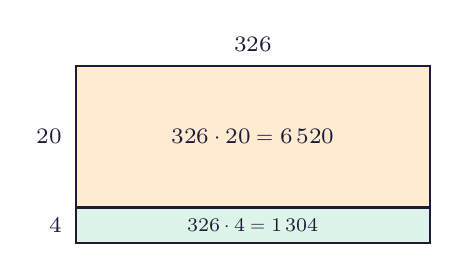
\begin{tikzpicture}[x=0.09cm,y=0.09cm,baseline=(current bounding box.north),font=\small]
  \fteil{0}{5}{50}{25}{px bar b}{$326\cdot20=6\,520$}
  \fteil{0}{0}{50}{5}{px bar c}{\scriptsize $326\cdot4=1\,304$}
  \foben{25}{25}{$326$}\flinks{0}{15}{$20$}\flinks{0}{2.5}{$4$}
\end{tikzpicture}}
% --- Division: 648:3 und 3712:8 (vier Schritte je Ziffer), Kreislauf der vier Schritte ---
\newcommand{\schrittbilddiv}{\begin{tikzpicture}[baseline=(current bounding box.north),font=\small]
  \node at (0.5,0) {6}; \node at (1.05,0) {4}; \node at (1.6,0) {8};
  \node[anchor=west] at (1.85,0) {$:3=\mathbf{2}\,1\,6$};
  \node at (0.0,-0.5) {$-$}; \node at (0.5,-0.5) {6};
  \draw[line width=0.6pt] (0.25,-0.76) -- (0.75,-0.76);
  \node at (0.5,-1.0) {0}; \node[text=pxblue,font=\small\bfseries] at (1.05,-1.0) {4};
  \node at (1.05,-1.5) {$-$}; \node at (1.6,-1.5) {$\ldots$};
  \draw[px mark] (0.3,0.22) rectangle (0.75,-0.22);
  \draw[px mark] (0.3,-0.28) rectangle (0.75,-0.72);
  \draw[px mark] (0.85,-0.78) rectangle (1.25,-1.22);
  \node[px bubble,text width=3.4cm,callout absolute pointer={(2.55,0.1)}] at (5.9,1.15) {\pxnum{1} \textbf{Teilen:} $6$ Hunderter auf $3$ verteilen: $6:3=2$\par\vspace{0.5mm}\begin{tikzpicture}[font=\scriptsize]\foreach \pxg in {0,1,2}{\draw[px bar,fill=white,line width=0.5pt] ({\pxg*1.0},0) rectangle ({\pxg*1.0+0.85},0.5); \pxsymH{\pxg*1.0+0.25}{0.25}\pxsymH{\pxg*1.0+0.6}{0.25}}\end{tikzpicture}};
  \node[px bubble,text width=3.4cm,callout absolute pointer={(0.78,-0.5)}] at (5.9,-0.55) {\pxnum{2} \textbf{Zurückmultiplizieren:} $2\cdot3=6$. Unter die $6$ schreiben};
  \node[px bubble,text width=3.4cm,callout absolute pointer={(0.78,-0.76)}] at (5.9,-1.45) {\pxnum{3} \textbf{Abziehen:} $6-6=0$};
  \node[px bubble,text width=3.4cm,callout absolute pointer={(1.28,-1.0)}] at (5.9,-2.3) {\pxnum{4} \textbf{Herunterholen:} die $4$ kommt neben die $0$. Weiter mit $4:3$};
\end{tikzpicture}}
\newcommand{\divrestbalken}{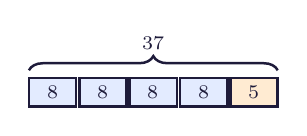
\begin{tikzpicture}[x=0.4cm,y=0.4cm,font=\scriptsize]
  \foreach \pxk in {0,1,2,3}{\fteil{\pxk*1.6}{0}{\pxk*1.6+1.5}{0.9}{px bar}{\scriptsize $8$}}
  \fteil{6.4}{0}{7.9}{0.9}{px bar b}{\scriptsize $5$}
  \draw[px brace] (0,1.15) -- (7.9,1.15) node[midway,above=1.2mm,px note,font=\scriptsize\bfseries]{$37$};
\end{tikzpicture}}
\newcommand{\schrittbilddivvier}{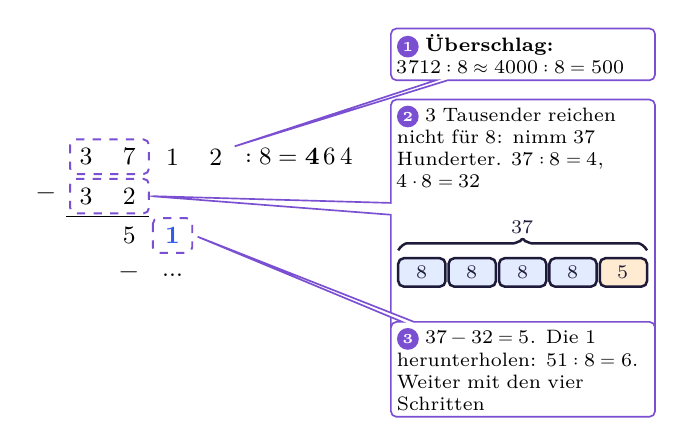
\begin{tikzpicture}[baseline=(current bounding box.north),font=\small]
  \node at (0.5,0) {3}; \node at (1.05,0) {7}; \node at (1.6,0) {1}; \node at (2.15,0) {2};
  \node[anchor=west] at (2.4,0) {$:8=\mathbf{4}\,6\,4$};
  \node at (0.0,-0.5) {$-$}; \node at (0.5,-0.5) {3}; \node at (1.05,-0.5) {2};
  \draw[line width=0.6pt] (0.25,-0.76) -- (1.3,-0.76);
  \node at (1.05,-1.0) {5}; \node[text=pxblue,font=\small\bfseries] at (1.6,-1.0) {1};
  \node at (1.05,-1.5) {$-$}; \node at (1.6,-1.5) {$\ldots$};
  \draw[px mark] (0.3,0.22) rectangle (1.3,-0.22);
  \draw[px mark] (0.3,-0.28) rectangle (1.3,-0.72);
  \draw[px mark] (1.35,-0.78) rectangle (1.85,-1.22);
  \node[px bubble,text width=3.2cm,callout absolute pointer={(2.35,0.12)}] at (6.05,1.3) {\pxnum{1} \textbf{Überschlag:} \mbox{$3712:8\approx4000:8=500$}};
  \node[px bubble,text width=3.2cm,callout absolute pointer={(1.32,-0.5)}] at (6.05,-0.75) {\pxnum{2} $3$ Tausender reichen nicht für $8$: nimm $37$ Hunderter. \mbox{$37:8=4$}, \mbox{$4\cdot8=32$}\par\vspace{0.5mm}\divrestbalken};
  \node[px bubble,text width=3.2cm,callout absolute pointer={(1.88,-1.0)}] at (6.05,-2.7) {\pxnum{3} \mbox{$37-32=5$}. Die $1$ herunterholen: \mbox{$51:8=6$}. Weiter mit den vier Schritten};
\end{tikzpicture}}
% Kreislauf der vier Divisionsschritte. Komplett-Kürzel, ca. 7,4 cm breit.
\newcommand{\divkreis}{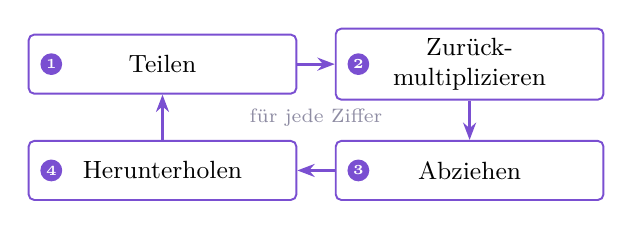
\begin{tikzpicture}[>={Stealth[length=2.2mm]},font=\small,baseline=(current bounding box.north),
  bx/.style={draw=pxpurple,fill=white,rounded corners=2pt,line width=0.7pt,minimum width=3.4cm,minimum height=0.75cm,align=center,text width=2.4cm,inner xsep=5mm},
  pxc/.style={circle,fill=pxpurple,text=white,inner sep=1pt,font=\tiny\bfseries}]
  \node[bx] (a) at (0,0) {Teilen}; \node[bx] (b) at (3.9,0) {Zurück\-multiplizieren};
  \node[bx] (c) at (3.9,-1.35) {Abziehen}; \node[bx] (d) at (0,-1.35) {Herunterholen};
  \foreach \pxn/\pxk in {1/a,2/b,3/c,4/d}{\node[pxc] at ([xshift=3mm]\pxk.west) {\pxn};}
  \draw[->,line width=1pt,pxpurple] (a) -- (b); \draw[->,line width=1pt,pxpurple] (b) -- (c);
  \draw[->,line width=1pt,pxpurple] (c) -- (d); \draw[->,line width=1pt,pxpurple] (d) -- (a);
  \node[font=\scriptsize,text=pxgray] at (1.95,-0.68) {für jede Ziffer};
\end{tikzpicture}}
% Rest deuten: 44 Bonbons in Tüten zu je 8 (5 volle Tüten, 4 übrig). Komplett-Kürzel, ca. 7,4 cm breit.
\newcommand{\restbild}{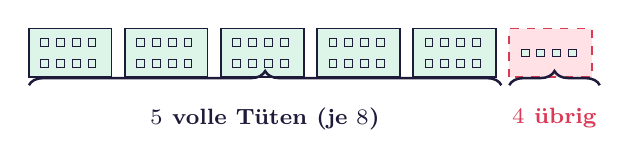
\begin{tikzpicture}[baseline=(current bounding box.north),font=\scriptsize]
  \foreach \pxt in {0,...,5}{%
    \pgfmathsetmacro{\pxx}{\pxt*1.22}
    \ifnum\pxt<5\draw[draw=pxink,fill=pxgreenlight,line width=0.6pt] (\pxx,0) rectangle ({\pxx+1.05},0.62);
      \foreach \pxa in {1,...,4}{\pxsymE{\pxx+\pxa*0.2}{0.44}\pxsymE{\pxx+\pxa*0.2}{0.18}}
    \else\draw[draw=pxred,fill=pxredlight,dashed,line width=0.6pt] (\pxx,0) rectangle ({\pxx+1.05},0.62);
      \foreach \pxa in {1,...,4}{\pxsymE{\pxx+\pxa*0.2}{0.31}}\fi}
  \draw[px brace] (0,-0.1) -- (6.0,-0.1) node[midway,below=1.6mm,px note]{$5$ volle Tüten (je $8$)};
  \draw[px brace] (6.1,-0.1) -- (7.25,-0.1) node[midway,below=1.6mm,px note,text=pxred]{$4$ übrig};
\end{tikzpicture}}
% --- Subtraktion: Gleiches Verändern (65-29 und 66-30 haben denselben Abstand). Komplett-Kürzel, ca. 7,7 cm breit. ---
\newcommand{\gleichesbild}{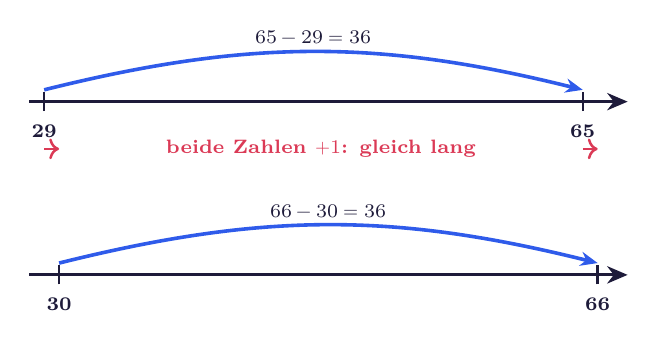
\begin{tikzpicture}[x=0.19cm,y=1cm,baseline=(current bounding box.north),font=\scriptsize]
  \foreach \pxy/\pxa/\pxb/\pxc/\pxd/\pxe in {2.2/1/37/29/65/{$65-29=36$},0/2/38/30/66/{$66-30=36$}}{%
    \begin{scope}[shift={(0,\pxy)}]
      \draw[px axis] (0,0) -- (40,0);
      \draw[px tick] (\pxa,-0.12) -- (\pxa,0.12); \draw[px tick] (\pxb,-0.12) -- (\pxb,0.12);
      \node[px lab,font=\scriptsize\bfseries] at (\pxa,-0.12) {\pxc}; \node[px lab,font=\scriptsize\bfseries] at (\pxb,-0.12) {\pxd};
      \draw[px jump] (\pxa,0.15) to[bend left=14] node[px jlab,midway,above=0.3mm,font=\scriptsize\bfseries]{\pxe} (\pxb,0.15);
    \end{scope}}
  \draw[->,line width=0.9pt,pxred] (1,1.6) -- (2,1.6); \draw[->,line width=0.9pt,pxred] (37,1.6) -- (38,1.6);
  \node[text=pxred,font=\scriptsize\bfseries] at (19.5,1.6) {beide Zahlen $+1$: gleich lang};
\end{tikzpicture}}
% --- Multiplikation: Verdoppeln und Halbieren (16*25 = 8*50: gleiche Fläche). Komplett-Kürzel, ca. 6,5 cm breit. ---
\newcommand{\halbierbild}{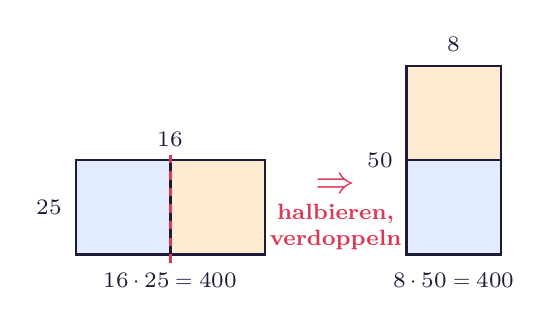
\begin{tikzpicture}[x=1cm,y=1cm,baseline=(current bounding box.north),font=\scriptsize]
  \fteil{0}{0}{1.2}{1.2}{px bar}{}\fteil{1.2}{0}{2.4}{1.2}{px bar b}{}
  \draw[dashed,line width=0.9pt,pxred] (1.2,-0.1) -- (1.2,1.3);
  \foben{1.2}{1.2}{$16$}\flinks{0}{0.6}{$25$}
  \node[px note,anchor=north] at (1.2,-0.1) {$16\cdot25=400$};
  \node[font=\Large,text=pxred] at (3.3,0.9) {$\Rightarrow$};
  \node[px note,text=pxred,align=center] at (3.3,0.35) {halbieren,\\verdoppeln};
  \fteil{4.2}{0}{5.4}{1.2}{px bar}{}\fteil{4.2}{1.2}{5.4}{2.4}{px bar b}{}
  \foben{4.8}{2.4}{$8$}\flinks{4.2}{1.2}{$50$}
  \node[px note,anchor=north] at (4.8,-0.1) {$8\cdot50=400$};
\end{tikzpicture}}
% --- Multiplikation: Über-und-unter (9*69 = 9*70 - 9). Komplett-Kürzel, ca. 7 cm breit. ---
\newcommand{\ueberuntenbild}{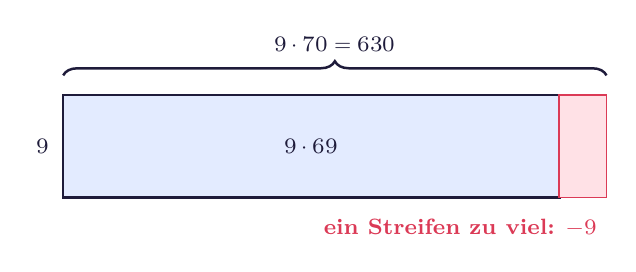
\begin{tikzpicture}[x=1cm,y=1cm,baseline=(current bounding box.north),font=\scriptsize]
  \fteil{0}{0}{6.3}{1.3}{px bar}{$9\cdot69$}
  \fteil{6.3}{0}{6.9}{1.3}{px hi}{}
  \draw[px brace] (0,1.55) -- (6.9,1.55) node[midway,above=1.6mm,px note]{$9\cdot70=630$};
  \flinks{0}{0.65}{$9$}
  \node[px note,text=pxred,anchor=north east] at (6.9,-0.15) {ein Streifen zu viel: $-9$};
\end{tikzpicture}}
% --- Strategie wählen: Entscheidungsweg mit drei Fragen und einer Endstrategie. Komplett-Kürzel, ca. 16 cm breit. ---
% \weichenbild{Frage 1}{Strategie 1}{Frage 2}{Strategie 2}{Frage 3}{Strategie 3}{Sonst-Strategie}
\newcommand{\weichenbild}[7]{\begin{tikzpicture}[>={Stealth[length=2.2mm]},font=\footnotesize,baseline=(current bounding box.north),
  q/.style={draw=pxpurple,fill=white,rounded corners=2pt,line width=0.7pt,text width=8.9cm,minimum height=0.68cm,align=left,inner xsep=7mm,inner ysep=2.5pt},
  s/.style={draw=pxink,fill=pxgreenlight,rounded corners=2pt,line width=0.8pt,minimum width=3.9cm,minimum height=0.68cm,font=\footnotesize\bfseries,align=center},
  pxc/.style={circle,fill=pxpurple,text=white,inner sep=1pt,font=\tiny\bfseries}]
  \node[q] (q1) at (5.0,0) {#1}; \node[s] (s1) at (14.4,0) {#2};
  \node[q] (q2) at (5.0,-1.1) {#3}; \node[s] (s2) at (14.4,-1.1) {#4};
  \node[q] (q3) at (5.0,-2.2) {#5}; \node[s] (s3) at (14.4,-2.2) {#6};
  \node[q,fill=pxorangelight] (q4) at (5.0,-3.3) {Passt keine Abkürzung?}; \node[s,fill=pxorangelight] (s4) at (14.4,-3.3) {#7};
  \foreach \pxi in {1,2,3,4}{\node[pxc] at ([xshift=3.5mm]q\pxi.west) {\pxi}; \draw[->,line width=0.9pt,pxgreen] (q\pxi.east) -- node[above,font=\scriptsize\bfseries,text=pxgreen]{ja} (s\pxi.west);}
  \foreach \pxi/\pxj in {1/2,2/3,3/4}{\draw[->,line width=0.9pt,pxred] (q\pxi.south) -- node[right,font=\scriptsize\bfseries,text=pxred]{nein} (q\pxj.north);}
\end{tikzpicture}}
% --- Überschlag: 68*31 wird zu 70*30. Komplett-Kürzel, ca. 6 cm breit. ---
\newcommand{\ueberschlagbild}{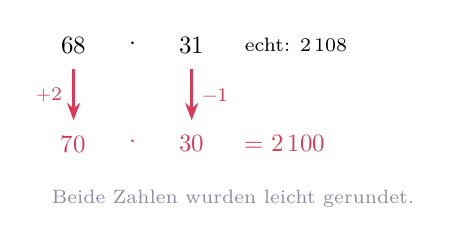
\begin{tikzpicture}[>={Stealth[length=2.2mm]},font=\small,baseline=(current bounding box.north)]
  \node at (0.4,0) {$68$}; \node at (1.15,0) {$\cdot$}; \node at (1.9,0) {$31$};
  \node[text=pxred,font=\small\bfseries] at (0.4,-1.25) {$70$}; \node[text=pxred] at (1.15,-1.25) {$\cdot$}; \node[text=pxred,font=\small\bfseries] at (1.9,-1.25) {$30$};
  \draw[->,line width=1pt,pxred] (0.4,-0.3) -- node[left,font=\scriptsize]{$+2$} (0.4,-0.95);
  \draw[->,line width=1pt,pxred] (1.9,-0.3) -- node[right,font=\scriptsize]{$-1$} (1.9,-0.95);
  \node[anchor=west,text=pxred,font=\small\bfseries] at (2.45,-1.25) {$=2\,100$};
  \node[anchor=west,font=\scriptsize] at (2.45,0) {echt: $2\,108$};
  \node[anchor=west,font=\scriptsize,text=pxgray] at (0,-1.95) {Beide Zahlen wurden leicht gerundet.};
\end{tikzpicture}}
% --- Division mit Teilquotienten: 936:24 als zwei Streifen (30 mal 24 und 9 mal 24). Komplett-Kürzel, ca. 6 cm breit. ---
\newcommand{\teilquotientbild}{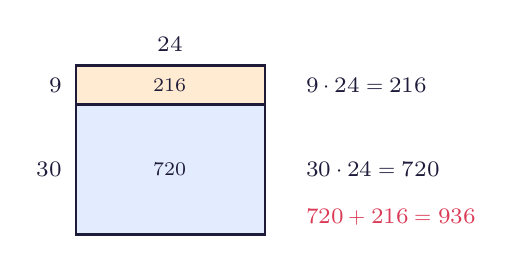
\begin{tikzpicture}[x=0.1cm,y=0.055cm,baseline=(current bounding box.north),font=\small]
  \fteil{0}{0}{24}{30}{px bar}{\scriptsize $720$}
  \fteil{0}{30}{24}{39}{px bar b}{\scriptsize $216$}
  \foben{12}{39}{$24$}\flinks{0}{15}{$30$}\flinks{0}{34.5}{$9$}
  \node[px note,anchor=west] at (28,15) {$30\cdot24=720$};
  \node[px note,anchor=west] at (28,34.5) {$9\cdot24=216$};
  \node[px note,anchor=west,text=pxred] at (28,4) {$720+216=936$};
\end{tikzpicture}}
